% use pdflatex -shell-escape slides.tex to compile
\documentclass[10pt]{beamer}
\usetheme{CambridgeUS}
%\usetheme[
%%% options passed to the outer theme
%    shownavsym          % show the navigation symbols
%]{AAUsimple}

\setbeamercolor{block title}{fg=gray!45!white,bg=darkred!80!black}
\overfullrule=5pt
% If you want to change the colors of the various elements in the theme, edit and uncomment the following lines
% Change the bar and sidebar colors:
%\setbeamercolor{AAUsimple}{fg=red!20,bg=red}
%\setbeamercolor{sidebar}{bg=red!20}
% Change the color of the structural elements:
%\setbeamercolor{structure}{fg=red}
% Change the frame title text color:
%\setbeamercolor{frametitle}{fg=blue}
% Change the normal text color background:
%\setbeamercolor{normal text}{fg=black,bg=gray!10}
% ... and you can of course change a lot more - see the beamer user
% manual.
\usepackage{animate}
\usepackage{tabularx}
\usepackage{epstopdf}
\usepackage{movie15}
\usepackage[utf8]{inputenc}
\usepackage[english]{babel}
\usepackage[T1]{fontenc}
% Or whatever. Note that the encoding and the font should match. If T1
% does not look nice, try deleting the line with the fontenc.
\usepackage{helvet}
\usepackage[helvet]{sfmath}
\usepackage{graphicx}
% For math font script
\usepackage[mathscr]{euscript}
\usepackage{algorithm,algorithmic}
\usepackage{color, xcolor}
\usepackage{tikz}
\usepackage{pgf}

% tikz setup for lattice graph
\usetikzlibrary{positioning,chains,fit,shapes,calc,snakes}
\usetikzlibrary{arrows,shadows,trees,automata}
% tikz animation
\usetikzlibrary{decorations.pathmorphing,through,backgrounds,petri}
\tikzset{
  basic/.style  = {draw, text width=2cm, drop shadow, font=\sffamily, rectangle},
  root/.style   = {basic, rounded corners=2pt, thin, align=center,
                   fill=red!30},
  level 2/.style = {basic, rounded corners=6pt, thin,align=center, fill=orange!30,
                   text width=8em},
  level 3/.style = {basic, thin, align=left, fill=pink!60, text width=8em},
  post/.style={->,>=stealth', thick},
  arc/.style={->,>=stealth' },
  node/.style={circle,draw,font=\sffamily\small},
  pile/.style={thin, ->, >=stealth', shorten <=2pt, shorten
  >=2pt},
  edge/.style={->, >=stealth', thin},
  edges/.style={->, shorten <=2pt, shorten >=2pt}
}
\newcommand{\Ispace}{\mathcal{I}}
\newcommand{\Rspace}{\mathcal{R}}
\newcommand{\sub}[1]{_{\mbox{\small #1}}}
\newcommand{\disk}{\sub{disk}}
\newcommand{\ident}{\sub{ident}}
\newcommand{\triv}{\sub{triv}}
\newcommand{\rect}{\sub{rect}}
\newcommand{\drect}{\sub{dblrect}}
\newcommand{\free}{\sub{free}}
\newcommand{\obst}{\sub{obst}}
\newcommand{\Rdisk}{\Rspace\disk}
\newcommand{\Rtriv}{\Rspace\triv}
\newcommand{\Rident}{\Rspace\ident}
\newcommand{\Rrect}{\Rspace\rect}
\newcommand{\Rdrect}{\Rspace\drect}
\newcommand{\Real}{\mathbb{R}}
\newcommand{\pow}{\operatorname{pow}}
\newcommand{\aabb}{\textsc{aabb}}
\newcommand{\drap}{\textsc{drap}}
\newcommand{\area}{\operatorname{area}}
\newcommand{\id}{{\rm id}}
\newcommand{\edge}[3]{{#1}\overset{#2}{\longrightarrow}{#3}}
\renewcommand{\L}{\Lambda}
\newcommand{\LT}{\Lambda^{\dagger}}
\newcommand{\G}{\mathcal{G}}
\newcommand{\sq}{\mathcal{S}}
\newcommand{\pv}{\mathcal{V}}
\newcommand{\A}{\G_{\L}}
\newcommand{\one}{^{(1)}}
\newcommand{\two}{^{(2)}}
\newcommand{\iii}{^{(i)}}
\newcommand{\ipo}{^{(i+1)}} 
% colored hyperlinks
% \newcommand{\chref}[2]{%
%   \href{#1}{{\usebeamercolor[bg]{AAUsimple}#2}}%
% }
\newcommand{\lgpath}[4]{{#1}\overset{#2}{\longrightarrow}{\cdots}\overset{#3}{\longrightarrow}{#4}}

\definecolor{scred}{RGB}{115,0,10}% dark red 
\definecolor{myblue}{RGB}{80,80,160}
\definecolor{mygreen}{RGB}{80,160,80}
\definecolor{mycyan}{RGB}{51,255,255}
\definecolor{myred}{RGB}{204,0,0}


\setbeamercolor{title}{fg=white, bg=scred}

\title[Ph.D. Proposal]{Constrained Geometric Approximation for Robot Planning and  Decentralized Formation Algorithm for Multi-Robot Systems}

\author[Yang Song]{
  \underline{Yang Song}\\
  Advisor: Jason M. O'Kane
}

\institute[
%  {\includegraphics[scale=0.2]{aau_segl}}\\ %insert a company, department or
%  university logo
USC
% Dept.\ of Computer Science and Engineering\\
  % University of South Carolina
] % optional - is placed in the bottom of the sidebar on every slide
{ % is placed on the bottom of the title page
  Dept. of Computer Science and Engineering\\
  University of South Carolina
  
  %there must be an empty line above this line - otherwise some unwanted space is added between the university and the country (I do not know why;( )
}

% specify a logo on the titlepage 
% institute command below
\pgfdeclareimage[height=1.5cm]{titlepagelogo}{sc_logo.pdf}
%\pgfdeclareimage[height=1.5cm]{titlepagelogo2}
\titlegraphic{% is placed on the bottom of the title page
  \pgfuseimage{titlepagelogo}
}

\begin{document}
% the titlepage
\begin{frame}
  \titlepage
\end{frame}
%%%%%%%%%%%%%%%%
\begin{frame}{Outlines}{}
\tableofcontents
\end{frame}
%%%%%%%%%%%%%%%%

\section{CGA for Robot Planning [ICRA 2012]}
\subsection[Overview]{Overview}
\begin{frame}{Constrained Geometric Approximation}
\begin{columns}
  \begin{column}{.65\textwidth}
    \begin{itemize}
    \item \textbf{Goal}:\\
    For an extremely simple robot with:
    \begin{itemize}
    \item computation limitations
    \item moving and sensing uncertainties
    \end{itemize}
    represent and reason about uncertainty in its own states efficiently.\\
    \item \textbf{Basic Idea}:\\
    Explicitly represent what the robot knows as an information state (\textit{I-state}).
    \item \textbf{Intuition}:\\
    Accelerate time-consuming operations by maintaining only an \textcolor[rgb]{1.00,0.00,0.00}{overapproximation} of the true
    I-state, and constraining this approximation
    to have a simple geometric form.\\
    \end{itemize}
  \end{column}
  \begin{column}{.35\textwidth}
    \begin{figure}
    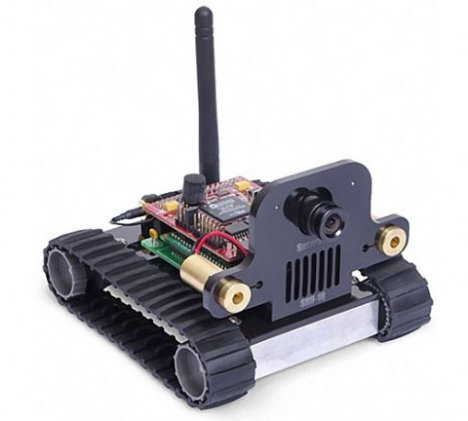
\includegraphics[scale=0.2]{figs/srvq.jpg}
    \end{figure}
    SRV-1 Surveyor Robot
  \end{column}
\end{columns}
\end{frame}

\begin{frame}{Prior Work}
Related work
\begin{itemize}
\item Probabilistic representations: J. van den Berg,
  P. Abbeel, and K. Goldberg (LQG-MP, IJRR 2011)
\item Minimal Representations: B. Tovar, L. Guilamo, S. M. LaValle (GNT, WAFR 2004)
\item Geometric overapproximation: J. M. O'Kane (ICRA 2011)
\end{itemize}
Contributions
\begin{itemize}
\item A careful formulation of the operations in the range space $\mathcal{R}$
\item Algorithms for double-rectangle range space $\mathcal{R}_{drect}$
\item A series of experiments for effectiveness comparison of different range spaces
\end{itemize}
\end{frame}

\begin{frame}{Robot Model}
Assume that current real state of the robot could not be observed directly.  The
robot could maintain an \emph{I-state} $\eta_k$, to make its decisions.
\begin{itemize}
\item State space: $X = \mathbb{R}^2$,  $X_{obt} \cup X_{free} \subseteq X$
\item Action space: $U = \mathbb{R}^2$, apply a bounded noise $\theta_k$ to the
  action $u_k \in U$
\item Set valued state transition function: $F(x, u)$
  \begin{equation}
    \label{eq:state-trans}
    F(x_k, u_k) = \left\{
      x_k + u_k + \theta_k
      \mid
      \theta_k \in \Theta(u_k)
    \right\} \cap X_{free}
  \end{equation}
  \begin{columns}
    \begin{column}{0.4\textwidth}
      \begin{figure}
        \centering
        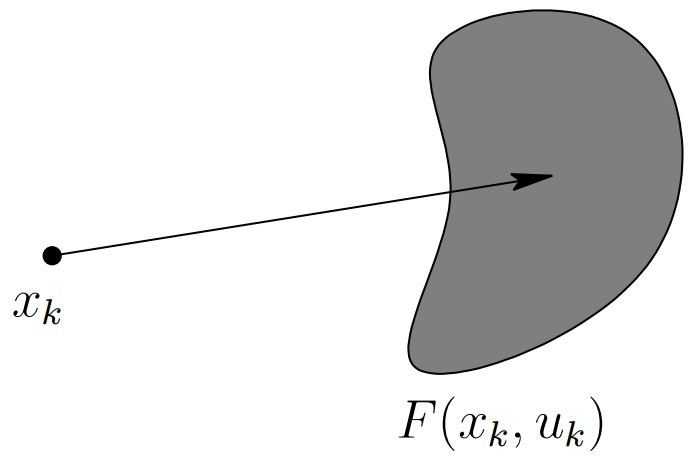
\includegraphics[scale=0.2]{figs/istate.jpg}
        \caption{\scriptsize{The transition of robot's state $x_k$ with
            uncertainty [\emph{Planning Algorithms}, S. LaValle, 2006].}}
      \end{figure}
    \end{column}
    \begin{column}{0.5\textwidth}
      \begin{figure}
        \centering
        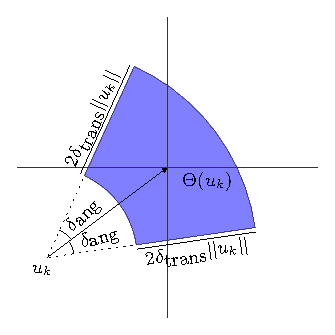
\includegraphics[scale=0.55]{figs/noisemodel}
        \caption{\scriptsize{The noise model $\Theta(u_k)$ involves bounded
            angular error $\delta_{ang}$ and bounded translational error
            $\delta_{trans}||u||$.}}
        \label{fig:noiseModel}
      \end{figure}
    \end{column}
  \end{columns}
\end{itemize}
\end{frame}

\begin{frame}{Robot Model (Cont'd)}
  \begin{itemize}
  \item Observation space: $Y = \mathbb{R}^2$
  \item Observation function: $h : X \to \pow(Y) $
  \item Observation Preimage: the set of states from which a given observation
    $y_k \in Y$ can be obtained
    \begin{equation}
      H(y_k) = \left\{ x_k \in X \mid y_k \in h(x_k), y_k \in Y \right\}
    \end{equation}
    
    \begin{figure}
      \centering
      \begin{tikzpicture}[scale=0.45]
        \draw[blue!20, fill=blue!20] (3, 3) circle (3);
        \draw[fill=violet] (3,3) circle (0.2);
        \draw[fill=red] (3,4.5) circle (0.1);
        \draw[fill=red] (3.2,1.7) circle (0.1);
        \draw[fill=red] (1,3) circle (0.1);
        \draw[fill=red] (2,0.5) circle (0.1);
        \draw[fill=red] (4,3.3) circle (0.1);
        \draw[fill=red] (4.4,4.8) circle (0.1);
      \end{tikzpicture}
      \caption{\scriptsize{The observation preimage set $H(y)$ (circle). Any states
          in this region (red points) can get observation of the landmark $y$
          (violet point).}}
    \end{figure}
  \end{itemize}
\end{frame}

\subsection[I-Space]{Information Space}
\begin{frame}{Information Space}
  \begin{definition}
  \small{An information state (I-state) $\eta$ is a set containing all possible
    states consistent with robot's sensor and action history.}
  \end{definition}
  \begin{definition}
  \small{The \emph{information space} (I-space) $\Ispace$ is the
  powerset of $X$, which contains all possible I-states.}
  \end{definition}
  \begin{columns}
    \begin{column}{0.4\textwidth}
       1. Action update function:
       $$X_{k+1}(\eta_{k}, u_k) =  \bigcup_{x_k \in \eta_k} F(x_k, u_k)$$
     \end{column}
    \begin{column}{0.5\textwidth}
      
\def\istate{
\coordinate (B1) at (5,3.5);
    \coordinate (B2) at (6,3.5);
    \coordinate (B3) at (5.5,2.5);
    \coordinate (B4) at (4.5,3);
    \fill[blue!20] (B1) -- (B2) -- (B3) -- (B4)  -- cycle;
    \path [draw] (B1) -- (B2);
    \path [draw] (B2) -- (B3);
    \path [draw] (B3) -- (B4);
    \path [draw] (B4) -- (B1);
    \node[] at (5.4, 3) {$\eta_k$};
    \draw[post] (5,3) -- (4,3.2)  node [above] {$u_k$};    
}

\def\istatef{
    \coordinate (A1) at (0,4);
    \coordinate (A2) at (1,4);
    \coordinate (A3) at (2.5,5);
    \coordinate (A4) at (3.5,3.5);
    \coordinate (A5) at (3,2);
    \coordinate (A6) at (1.75,2);
    \path [draw] (A1) -- (A2);
    \path [draw] (A2) -- (A3);
    \path [draw] (A3) -- (A4);
    \path [draw] (A4) -- (A5);
    \path [draw] (A5) -- (A6);
    \path [draw] (A6) -- (A1);
    \fill[blue!20] (A1) -- (A2) -- (A3) -- (A4)  -- (A5) --(A6) -- cycle;
    \node[] at (1.5,3.5) {$X_{k+1}(\eta_k, u_k)$};
  
}

\def\istateo{
    \coordinate (A1) at (0,4);
    \coordinate (A2) at (1,4);
    \coordinate (A3) at (2.5,5);
    \coordinate (A4) at (3.5,3.5);
    \coordinate (A5) at (3,2);
    \coordinate (A6) at (1.75,2);
    \path [draw] (A1) -- (A2);
    \path [draw] (A2) -- (A3);
    \path [draw] (A3) -- (A4);
    \path [draw] (A4) -- (A5);
    \path [draw] (A5) -- (A6);
    \path [draw] (A6) -- (A1);
    
    \fill[fill=blue!20](A1) -- (A2) -- (A3) -- (A4)  -- (A5) --(A6) -- cycle;
    \node[] at (1.5,3.5) {$X_{k+1}(\eta_k, u_k)$};
    \coordinate (L) at (1,2);
    \draw[fill=blue] (L) circle (0.1);
    \node[] at (1.2,1.6) {$H(y_k)$};
    \draw[blue] (L) circle (1.5);
    \node[] at (1.8,2.75) {$\eta_{k+1}$};
}
        
\begin{tikzpicture}[scale=0.75]
    \useasboundingbox (0,0) rectangle (5,5.5);         
    \istatef        
    \istate
\end{tikzpicture}
    \end{column}
  \end{columns}
\end{frame}

\begin{frame}{Information Space}
  \begin{definition}
    \small{An information state (I-state) $\eta$ is a set containing all possible
      states consistent with robot's sensor and action history.}
  \end{definition}
  \begin{definition}
    \small{The \emph{information space} (I-space) $\Ispace$ is the
      powerset of $X$, which contains all possible I-states.}
  \end{definition}
  \begin{columns}
    \begin{column}{0.4\textwidth}
      2. Observation update function:
      $$\eta_{k+1} =   X_{k+1}(\eta_{k}, u_k) \cap H(y_{k})$$
    \end{column}
    \begin{column}{0.5\textwidth}
      \begin{animateinline}[
  begin={%
    \begin{tikzpicture}%
      [scale=0.75,
      post/.style={->,>=stealth', semithick, draw=blue!50},
      node/.style={circle,fill=red!20,draw,font=\sffamily\small}]%
      \useasboundingbox (0,0) rectangle (5,5.5);
    },
    end={\end{tikzpicture}}
  ]{10}
  \coordinate (A1) at (0,4);
  \coordinate (A2) at (1,4);
  \coordinate (A3) at (2.5,5);
  \coordinate (A4) at (3.5,3.5);
  \coordinate (A5) at (3,2);
  \coordinate (A6) at (1.75,2);
  \path [draw] (A1) -- (A2);
  \path [draw] (A2) -- (A3);
  \path [draw] (A3) -- (A4);
  \path [draw] (A4) -- (A5);
  \path [draw] (A5) -- (A6);
  \path [draw] (A6) -- (A1);
  \fill[blue!20] (A1) -- (A2) -- (A3) -- (A4)  -- (A5) --(A6) -- cycle;               \node[] at (1.5,3.5) {$X_{k+1}(\eta_k, u_k)$};
  \coordinate (L) at (3,3.5);
  \draw[fill=blue] (L) circle (0.1);
  \node[] at (3.7,4.2) {$H(y_k)$};
  \draw[blue] (L) circle (1.5);
  %%%% new frame %%%%
  \newframe*
  \multiframe{10}{}{ 
    \coordinate (A1) at (0,4);
    \coordinate (A2) at (1,4);
    \coordinate (A3) at (2.5,5);
    \coordinate (A4) at (3.5,3.5);
    \coordinate (A5) at (3,2);
    \coordinate (A6) at (1.75,2);
    \coordinate (L) at (3,3.5);
    
    \draw[fill=blue] (L) circle (0.1);
    \node[] at (2.5,3) {$\eta_{k+1}$};
    \begin{scope}
      \clip (A1) -- (A2) -- (A3) -- (A4)  -- (A5) -- (A6) -- cycle;
      \draw[blue, fill=blue!20] (L) circle (1.5);
    \end{scope}
    \node[] at (2.5,3.4) {$\eta_{k+1}$};
    \draw[blue] (2.55,4.95) -- (A4);
    \draw[blue] (A4) -- (A5);
  }
\end{animateinline}
    \end{column}
  \end{columns}  
 \end{frame}

\begin{frame}{Simulation: Navigation Task}
 \begin{block}{Ultimate Objective} 
   Form a plan $\pi$ for the robot to execute using the information available in
   the information space.
 \end{block}

\textbf{In a navigation task, we assume:}
\begin{itemize}
\item A point robot follows predefined waypoints guided by centroid point of the
  approximated I-state
\item Robot can detect presence but not distance to the landmarks
\item Landmarks are pseudo-randomly generated
\item Initial I-state $A(\eta_0)$ is given
\end{itemize}
\end{frame}

\begin{frame}{Example}{Navigation Task using I-state}
  \begin{center}
    \includemovie[toolbar,poster,autoplay]{12cm}{6cm}{videos/clutter_istate.mp4}
  \end{center}
\end{frame} 

%%%%%%%%%%%%%%%%%%%%%%%%%%%%%%%%%%%%%%%%%%%%%%%%%%%%%%%%%%%%%%%%%%%%%%%%%%%%%
\subsection[Range Space]{Contribution: Range Space}
\begin{frame}{Contribution: Range Space}
  \begin{definition}{\textbf{A range space}}
    $\mathcal{R} \subseteq \mathcal{I}$ is a set of I-states, equipped with two
    operations:
  \end{definition}
  \begin{columns}
    \begin{column}{.5\textwidth}
      \begin{enumerate}
      \item \emph{Approximate action update function} $T: \mathcal{R} \times U \to
        \mathcal{R}$:
        $$\bigcup_{x_k \in \eta_k} F(x_k, u_k) \subseteq T(A(\eta_k), u_k)$$
      \item \emph{Approximate observation update function} $O: \mathcal{R} \times
        Y \to \mathcal{R}$:
        $$\eta_k \cap H(y_k) \subseteq O(A(\eta_k), u_k)$$
      \end{enumerate}
      \textcolor{scred}{Intuition: always overapproximate I-state:
        $\eta_k \subseteq A(\eta_k)$}
    \end{column}
    \begin{column}{.4\textwidth}
    \begin{figure}
      \begin{tikzpicture}[scale=0.75]
      \begin{scope}
        \clip (0,0) rectangle (4,4);
        \draw[fill=green!20] (0,0) circle (3cm);
        \draw[fill=white] (0,0) circle (1cm);  
      \end{scope}
      \draw[blue] (0,0) -- (3,0) -- (3,3) -- (0,3) -- (0,0);
      \draw[red]  (1.5,1.5) circle (2.13cm);
      \node at (1.3,1.3) {$\eta_k$};    
    \end{tikzpicture} 
    \caption{\scriptsize{An \emph{I-state} $\eta_k$ (shaded region),
        overapproximations $A(\eta_k)$ using disk (red circle) and rectangle
        (blue). }}
    \end{figure}
  \end{column}
\end{columns}
\end{frame}

\begin{frame}{Example}{Rectangle Approximation of I-state}
  \begin{center}
    \includemovie[toolbar,poster,autoplay]{12cm}{6cm}{videos/clutter_rect.mp4}
  \end{center}
\end{frame}

\begin{frame}{Limitation}{Rectangle Approximation of I-state}
  \textbf{Problem: approximation accuracy}
   \begin{columns}
    \begin{column}{0.45\textwidth}
      \begin{figure}
        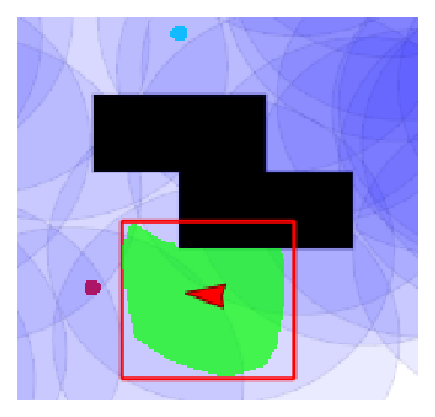
\includegraphics[width=0.5\linewidth]{figs/rect_approx}
      \end{figure}
    \end{column}
    \begin{column}{0.45\textwidth}
      \begin{figure}
        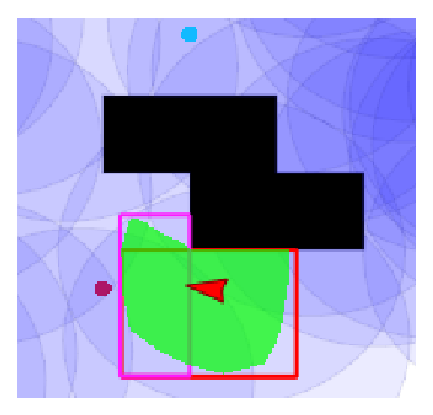
\includegraphics[width=0.5\linewidth]{figs/dbrect_approx}
      \end{figure}
    \end{column}
  \end{columns}
\end{frame}

\subsubsection[Double-Rectangle Range Space]{Double-Rectangle Range Space}
\begin{frame}{Double-Rectangle approximated I-state}
  To improve the approximation quality for non-convex \emph{I-states}, we
  proposed:
  \begin{itemize}
  \item a novel range space of \textcolor[rgb]{1.00,0.00,0.00}{double-rectangle}
    \begin{equation}
      \mathcal{R}_{drect} = \{ R_1 \cup R_2 \mid R_1, R_2 \in \mathcal{R}_{rect} \}
    \end{equation}
  \item an algorithm to overapproximate a polygon using double-rectangle
    \begin{center}
      \def\polygon{
    \coordinate (A1) at (0,0.5);
    \coordinate (A2) at (1,2);
    \coordinate (A3) at (1.5,1.2);
    \coordinate (A4) at (2.5,3);
    \coordinate (A5) at (3,2);
    \coordinate (A6) at (4,1.5);
    \coordinate (A7) at (2.2,0);
    % \node [left] at (A1) {$A_1$};
    % \node [above] at (A2) {$A_2$};
    % \node [below] at (A3) {$A_3$};
    % \node [right] at (A4) {$A_4$};
    % \node [right] at (A5) {$A_5$};
    % \node [right] at (A6) {$A_6$};
    % \node [below] at (A7) {$A_7$};
    \path [draw] (A1) -- (A2);
    \path [draw] (A2) -- (A3);
    \path [draw] (A3) -- (A4);
    \path [draw] (A4) -- (A5);
    \path [draw] (A5) -- (A6);
    \path [draw] (A6) -- (A7);
    \path [draw] (A7) -- (A1);
    %\coordinate [name intersections  ={of= A1A2 and A2A3,by = intersect-1}];
    %\fill[violet!20] (A1) -- (intersect-1) -- (A3) -- cycle;
    \fill[violet!20] (A1) -- (A2) -- (A3) -- (A4) --(A5) -- (A6) -- (A7) -- cycle;
    \foreach \Index in {1, 2, 3, 4, 5, 6, 7} 
    {
        \draw[violet] (A\Index) circle (0.025) ;
    }
}

  \begin{animateinline}
    [
        begin={%
          \begin{tikzpicture}%
           [post/.style={->,>=stealth', semithick, draw=blue!50},
            node/.style={circle,fill=red!20,draw,font=\sffamily\small}]%
          },
          end={\end{tikzpicture}}
        ]{10}
        \polygon
        \newframe*
        \multiframe{10}{}{ 
          \polygon
          \coordinate (C) at (2,1.3);
          \draw[fill=orange] (C) circle (0.04);
          \draw[green] (A2) -- (A3);
        }
        \newframe*
        \multiframe{10}{}{ 
          \polygon
          \coordinate (C) at (2,1.3);
          \draw[fill=orange] (C) circle (0.04);
          \coordinate (B1) at (1,1.2);
          \coordinate (B2) at (2,2);
          \draw[blue] (B1) rectangle (B2);
          \draw[green] (A2) -- (A3);
          \draw[green] (A3) -- (A4);
        }
        \newframe*
        \multiframe{10}{}{ 
          \polygon
          \coordinate (C) at (2,1.3);
          \draw[fill=orange] (C) circle (0.04);
          \coordinate (B1) at (1,1.2);
          \coordinate (B2) at (2,2);
          \draw[blue] (B1) rectangle (B2);
          \draw[red] (A3) rectangle (A4);
          \draw[green] (A2) -- (A3);
          \draw[green] (A3) -- (A4);
          \draw[green] (A4) -- (A5);
        }
        \newframe*
        \multiframe{10}{}{ 
          \polygon
          \coordinate (C) at (2,1.3);
          \draw[fill=orange] (C) circle (0.04);
          \coordinate (B1) at (1,1.2);
          \coordinate (B2) at (2,2);
          \draw[blue] (B1) rectangle (B2);
          \coordinate (B3) at (3,3);
          \draw[red] (A3) rectangle (B3);
          \draw[green] (A2) -- (A3);
          \draw[green] (A3) -- (A4);
          \draw[green] (A4) -- (A5);
          \draw[green] (A5) -- (A6);
        }
        \newframe*
        \multiframe{10}{}{ 
          \polygon
          \coordinate (C) at (2,1.3);
          \draw[fill=orange] (C) circle (0.04);
          \coordinate (B1) at (1,1.2);
          \coordinate (B4) at (4,2);
          \draw[blue] (B1) rectangle (B4);
          \coordinate (B3) at (3,3);
          \draw[red] (A3) rectangle (B3);
          \draw[green] (A2) -- (A3);
          \draw[green] (A3) -- (A4);
          \draw[green] (A4) -- (A5);
          \draw[green] (A5) -- (A6);
          \draw[green] (A6) -- (A7);
        }
        \newframe*
        \multiframe{10}{}{ 
          \polygon
          \coordinate (C) at (2,1.3);
          \draw[fill=orange] (C) circle (0.04);
          \coordinate (B5) at (1,0);
          \coordinate (B4) at (4,2);
          \draw[blue] (B5) rectangle (B4);
          \coordinate (B3) at (3,3);
          \draw[red] (A3) rectangle (B3); 
          \draw[green] (A2) -- (A3);
          \draw[green] (A3) -- (A4);
          \draw[green] (A4) -- (A5);
          \draw[green] (A5) -- (A6);
          \draw[green] (A6) -- (A7);
          \draw[green] (A7) -- (A1);
        }
        \newframe*
        \multiframe{10}{}{ 
          \polygon
          \coordinate (C) at (2,1.3);
          \draw[fill=orange] (C) circle (0.04);
          \coordinate (B6) at (0,0);
          \coordinate (B4) at (4,2);
          \draw[blue] (B6) rectangle (B4);
          \coordinate (B3) at (3,3);
          \draw[red] (A3) rectangle (B3);
          \draw[green] (A2) -- (A3);
          \draw[green] (A3) -- (A4);
          \draw[green] (A4) -- (A5);
          \draw[green] (A5) -- (A6);
          \draw[green] (A6) -- (A7);
          \draw[green] (A7) -- (A1);
          \draw[green] (A1) -- (A2);
        }
  \end{animateinline}
    \end{center} 
  \end{itemize}
  
\end{frame}

\begin{frame}{Operations on Double-Rectangle Range Space}
  For a double rectangle approximated \emph{I-state} $A(\eta_k) = R_1 \cup R_2$:
  \begin{itemize}
  \item \small{Action Update:\\$T_{drect}\left(A(\eta_k), u_k \right)=DRAP\left(X_{free} \cap [A(\eta_k) \oplus \{ u_k \} \oplus DRAP\left(\Theta(u_k)\right)]\right)$}
  \item \small{Observation Update:\\$O_{drect}\left(A(\eta_k), y_k\right)=AABB\left(H(y_k) \cap R_1\right)\cup AABB\left(H(y_k) \cap R_2\right)$}
  \end{itemize}
  \begin{center}  
    
\def\obs{
    \coordinate (B1) at (0,0);
    \coordinate (B2) at (1,0);
    \coordinate (B3) at (1,2);
    \coordinate (B4) at (0,2);
    \fill[fill=gray] (B1) -- (B2) --(B3) -- (B4) -- cycle; 
}

\def\obst{
    \coordinate (C1) at (2.5,0.5);
    \coordinate (C2) at (4.5,0.5);
    \coordinate (C3) at (4.5,1.5);
    \coordinate (C4) at (2.5,1.5);
    \fill[fill=gray] (C1) -- (C2) --(C3) -- (C4) -- cycle; 
}

\def\dbrect{
    \draw[blue, fill=blue!20] (1.7, 3) rectangle (2.6,4);
    \draw[blue, fill=blue!20] (1.3,2.8) rectangle (3,3.5);
    \draw[post] (2,3.4) -- (1.8, 2) node [right] {$u_k$};
    \node [below] at (2.5, 3.4) {\small{$A(\eta_k)$}};
}

\def\dbrectf{
    \draw[blue, fill=blue!20] (1,0.3) rectangle (2.3, 2);
    \draw[blue, fill=blue!20] (1,-0.5) rectangle (3.2, 0.5);
    \node [below] at (1.75, 1.85) {$X_{k+1}$};
}

\def\landmark{
    \coordinate (L) at (3, 0);
    \draw[violet] (L) circle (1.5);
    \draw[fill=orange] (L) circle (0.1);
    \node [below] at (3.75, 0) {\small{$H(y_k)$}};
}

\def\newdbrect{
    \draw[red] (1.5,-0.5) rectangle (2.3,1.35);
    \draw[red] (1.5,-0.5) rectangle (3.2, 0.5);
}

\def\newdbrectf{
    \draw[red, fill=red!20] (1.5,-0.5) rectangle (2.3,1.35);
    \draw[red, fill=red!20] (1.5,-0.5) rectangle (3.2, 0.5);
    \node at (2.2,0) {\small{$A(\eta_{k+1})$}};
}

\begin{animateinline}[
    begin={%
      \begin{tikzpicture}[scale=0.7]%
        [post/.style={->,>=stealth', semithick, draw=blue!50},
        node/.style={circle,fill=red!20,draw,font=\sffamily\small}]%
        \useasboundingbox (0,-2) rectangle (5,5);
      },
      end={\end{tikzpicture}}
    ]{10}
    \obs
    \obst
    \dbrect
    \newframe*
    \multiframe{10}{}{ 
      \obs
      \obst
      \dbrectf
    } 
    \newframe*
    \multiframe{10}{}{ 
      \obs
      \obst
      \dbrectf
      \landmark
    }
    \newframe*
    \multiframe{10}{}{ 
      \obs
      \obst
      \dbrectf
      \newdbrect
      \landmark
    }
    \newframe*
    \multiframe{10}{}{ 
      \obs
      \obst
      \newdbrectf
    }
  \end{animateinline}
      
  \end{center}
\end{frame}

\begin{frame}{Simulation}{Double-Rectangle Approximation of I-state}
  \begin{center}
    \includemovie[toolbar,poster,autoplay]{12cm}{6cm}{videos/clutter_dbrect.mp4}
  \end{center}
\end{frame} 

%%%%%%%%%%%%%%%%%%%%%%%%%%%%%%%%%%%%%%%%%%%%%%%%%%%%%%%%%%%%%%%%%%%%%%%%%%%%

\subsection[Experiments]{Experiments and Conclusions}
\begin{frame}{Experimental Results}{Success Rate}
 \small{Comparison with using the true I-state, we conducted experiments using 3
 environments, and 3 range spaces $\mathcal{R}_{disk}$, $\mathcal{R}_{rect}$,
 and  $\mathcal{R}_{drect}$. \\
 In each environment we collect the success rate of completing the navigation
 task. 
 \begin{enumerate}
 \item The number of landmarks $N$: between $5$ and $250$ in increments of 5
 \item For each $N$, run the experiment 15 trials with different landmark
   distributions by assigning distinct random seeds
 \end{enumerate}
}
\begin{figure}
  \centering
  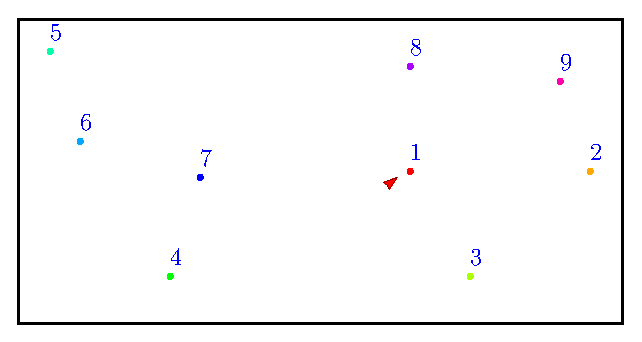
\includegraphics[width=0.65\textwidth]{figs/blank}
\end{figure}
\end{frame}

\begin{frame}{Experimental Results}{Success Rate (Cont'd)}
 \small{Comparison with using the true I-state, we conducted experiments using 3
 environments, and 3 range spaces $\mathcal{R}_{disk}$, $\mathcal{R}_{rect}$,
 and  $\mathcal{R}_{drect}$. \\
 In each environment we collect the success rate of completing the navigation
 task. 
 \begin{enumerate}
 \item The number of landmarks $N$: between $5$ and $250$ in increments of 5
 \item For each $N$, run the experiment 15 trials with different landmark
   distributions by assigning distinct random seeds
 \end{enumerate}
}
\begin{figure}
  \centering
  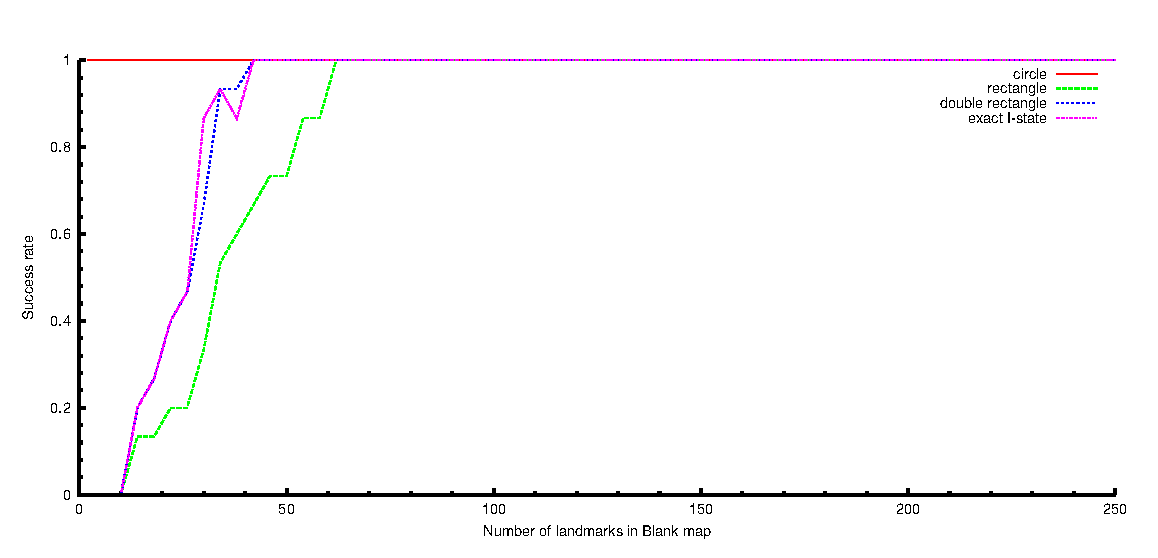
\includegraphics[width=0.71\textwidth]{figs/exp_num_blank}
\end{figure}
\end{frame}

\begin{frame}{Experimental Results}{Success Rate (Cont'd)}
 \small{Comparison with using the true I-state, we conducted experiments using 3
 environments, and 3 range spaces $\mathcal{R}_{disk}$, $\mathcal{R}_{rect}$,
 and  $\mathcal{R}_{drect}$. \\
 In each environment we collect the success rate of completing the navigation
 task. 
 \begin{enumerate}
 \item The number of landmarks $N$: between $5$ and $250$ in increments of 5
 \item For each $N$, run the experiment 15 trials with different landmark
   distributions by assigning distinct random seeds
 \end{enumerate}
}
\begin{figure}
  \centering
  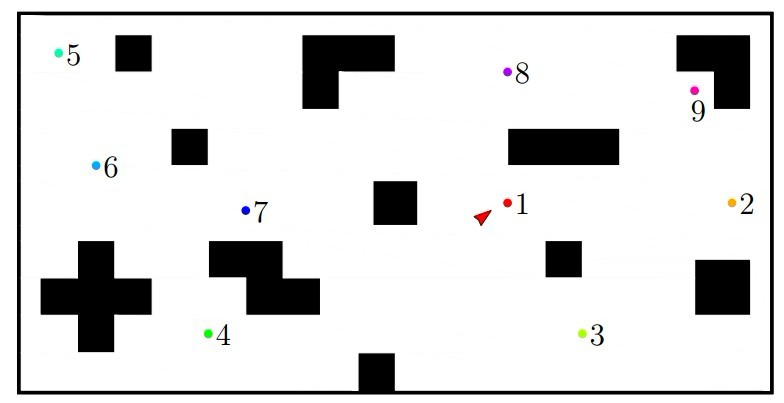
\includegraphics[width=0.65\textwidth]{figs/clutter}
\end{figure}
\end{frame}

\begin{frame}{Experimental Results}{Success Rate (Cont'd)}
 \small{Comparison with using the true I-state, we conducted experiments using 3
 environments, and 3 range spaces $\mathcal{R}_{disk}$, $\mathcal{R}_{rect}$,
 and  $\mathcal{R}_{drect}$. \\
 In each environment we collect the success rate of completing the navigation
 task. 
 \begin{enumerate}
 \item The number of landmarks $N$: between $5$ and $250$ in increments of 5
 \item For each $N$, run the experiment 15 trials with different landmark
   distributions by assigning distinct random seeds
 \end{enumerate}
}
\begin{figure}
  \centering
  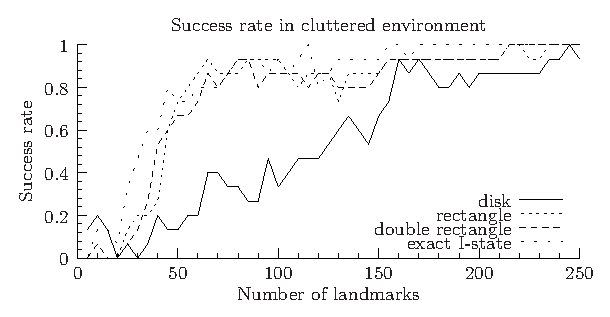
\includegraphics[width=0.71\textwidth]{figs/exp_num_clutter}
\end{figure}
\end{frame}

\begin{frame}{Experimental Results}{Success Rate (Cont'd)}
 \small{Comparison with using the true I-state, we conducted experiments using 3
 environments, and 3 range spaces $\mathcal{R}_{disk}$, $\mathcal{R}_{rect}$,
 and  $\mathcal{R}_{drect}$. \\
 In each environment we collect the success rate of completing the navigation
 task. 
 \begin{enumerate}
 \item The number of landmarks $N$: between $5$ and $250$ in increments of 5
 \item For each $N$, run the experiment 15 trials with different landmark
   distributions by assigning distinct random seeds
 \end{enumerate}
}
\begin{figure}
  \centering
  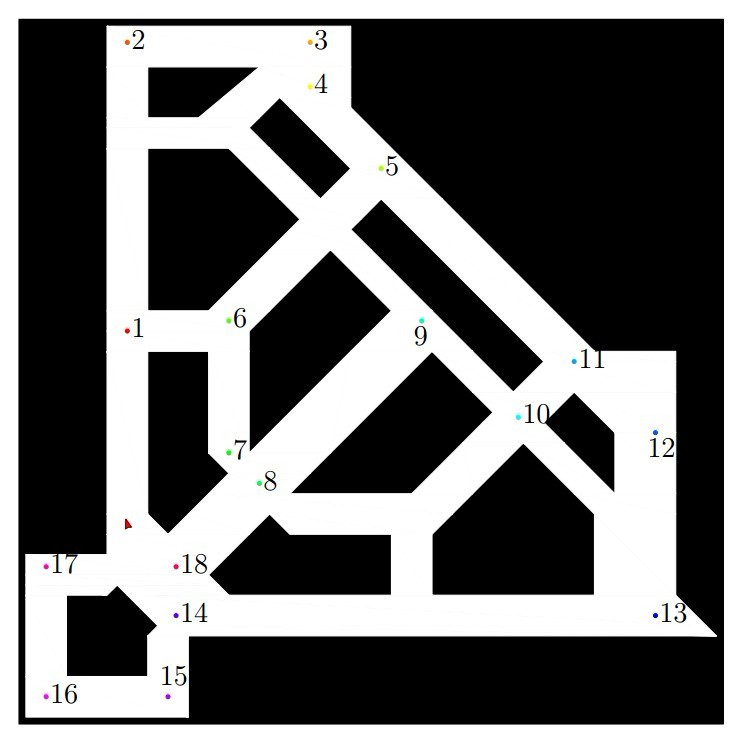
\includegraphics[width=0.33\textwidth]{figs/office}
\end{figure}
\end{frame}

\begin{frame}{Experimental Results}{Success Rate (Cont'd)}
 \small{Comparison with using the true I-state, we conducted experiments using 3
 environments, and 3 range spaces $\mathcal{R}_{disk}$, $\mathcal{R}_{rect}$,
 and  $\mathcal{R}_{drect}$. \\
 In each environment we collect the success rate of completing the navigation
 task. 
 \begin{enumerate}
 \item The number of landmarks $N$: between $5$ and $250$ in increments of 5
 \item For each $N$, run the experiment 15 trials with different landmark
   distributions by assigning distinct random seeds
 \end{enumerate}
}
\begin{figure}
  \centering
  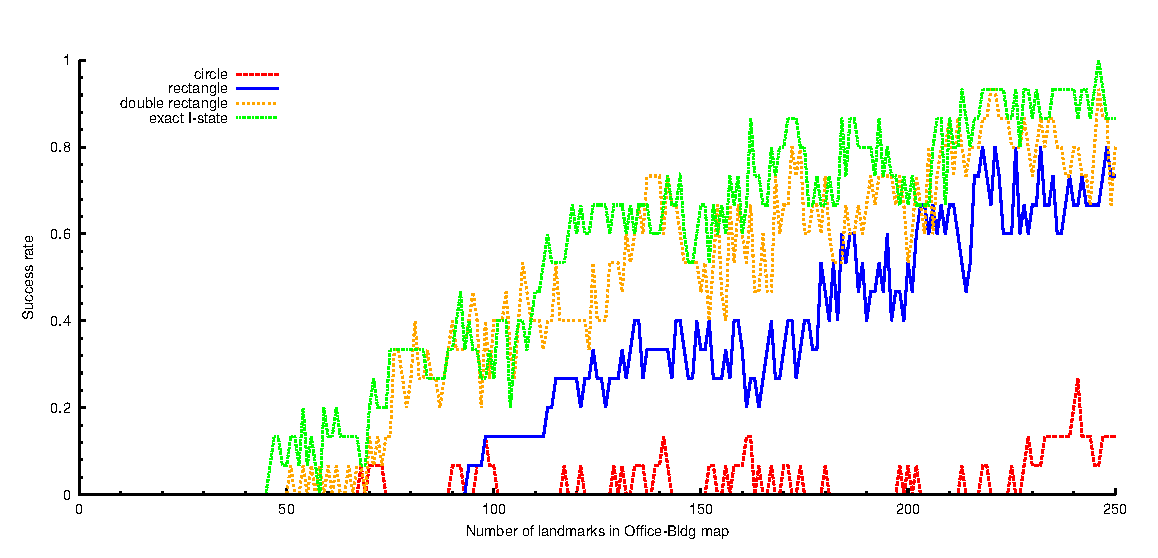
\includegraphics[width=0.71\textwidth]{figs/exp_num_cse}
\end{figure}
\end{frame}

\begin{frame}{Experimental Results}{Computation Time}
  For each environment, we
  \begin{itemize}
  \item randomly place $N = 300$ landmarks 
  \item run the  experiments $10$ times
  \end{itemize} 
  \begin{block}{}
    We compare the average time (in seconds) required to compute the approximated
    \emph{I-state} compared to the high-fidelity polygonal representation of the
    exact \emph{I-state}.
  \end{block}
\begin{table}
  \footnotesize\centering
    \begin{tabular}{cccc} 
    \hline
    Range & \multicolumn{3}{c}{Computation Time (s)}  \\
    Space & Obstacle-free & Obstacle-cluttered & Office-like\\
    \hline
    $\mathcal{R}_{disk}$ & 0.163  & 0.162   & 0.292  \\ 
    \hline
    $\mathcal{R}_{rect}$ & 0.396   & 0.441  & 0.415  \\
    \hline
    $\mathcal{R}_{dblrect}$ & 1.021  & 1.122  & 1.491  \\
    \hline
    $\mathcal{I}$ & 10.074  & 10.218  & 26.895  \\
    \hline
    \end{tabular}
    \caption{\scriptsize{Average computation time in three environments.}}
\end{table}
\end{frame}

\begin{frame}{Experimental Results}{Approximation Ratio}
  For each environment, we
  \begin{itemize}
  \item randomly place $N = 300$ landmarks 
  \item run the  experiments $10$ times
  \end{itemize} 
  \begin{block}{}
    We compare the average approximation ratio of using each approximation methods
    to approximate  the true \emph{I-state}
    $$\frac{1}{k} \sum_{i=1}^k \frac{\text{AREA}(\eta_i)}{\text{AREA}(A(\eta_i))}$$
  \end{block}
\begin{table}
  \footnotesize\centering
    \begin{tabular}{cccc} 
    \hline
    Range  & \multicolumn{3}{c}{Approximation  Ratio}  \\
    Space  & Obstacle-free & Obstacle-cluttered & Office-like\\
    \hline
    $\mathcal{R}_{disk}$ & 0.155  & 0.155   & 0.220 \\ 
    \hline
    $\mathcal{R}_{rect}$  & 0.642   & 0.632  & 0.661 \\
    \hline
    $\mathcal{R}_{dblrect}$ & 0.684 & 0.691  & 0.720 \\
    \hline
    $\mathcal{I}$ & 1.000  & 1.000  & 1.000 \\
    \hline
    \end{tabular}
    \caption{\scriptsize{Average approximation ratio in three environments.}}
\end{table}

\end{frame}

\begin{frame}{Conclusions}
  \begin{enumerate}
  \item CGA is effective for representing a robot's uncertain information about
    the current state
  \item The form of double-rectangle is more accurate in approximating the non-convex
    \emph{I-state}
  \item The robot can complete the navigation task using approximated I-state with
    low approximation accuracy
  \end{enumerate}
\end{frame}

\section{Distributed Multi-Robot Formation [ICRA 2014]}
\subsection[Overview]{Overview}
\begin{frame}{Related Work}{Formation using virtual force}
   \begin{columns}[T] 
    \begin{column}{.45\textwidth}
      \scriptsize{W. Spears, D. Spears, J. Hamann and R. Heil, 2004}
      \begin{figure}
        \centering
        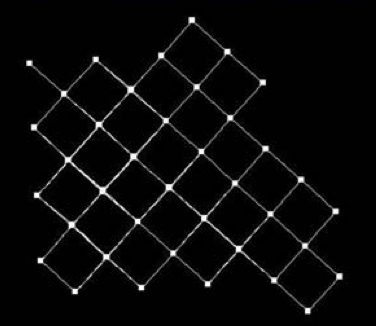
\includegraphics[height=1in]{figs/spears1.png}
      \end{figure}
    \end{column}%
    \begin{column}{.45\textwidth}
      \scriptsize{I. Navarro, J. Pugh, A. Martinoli, and
        F. Matia, 2008}
      \begin{figure}
        \centering
        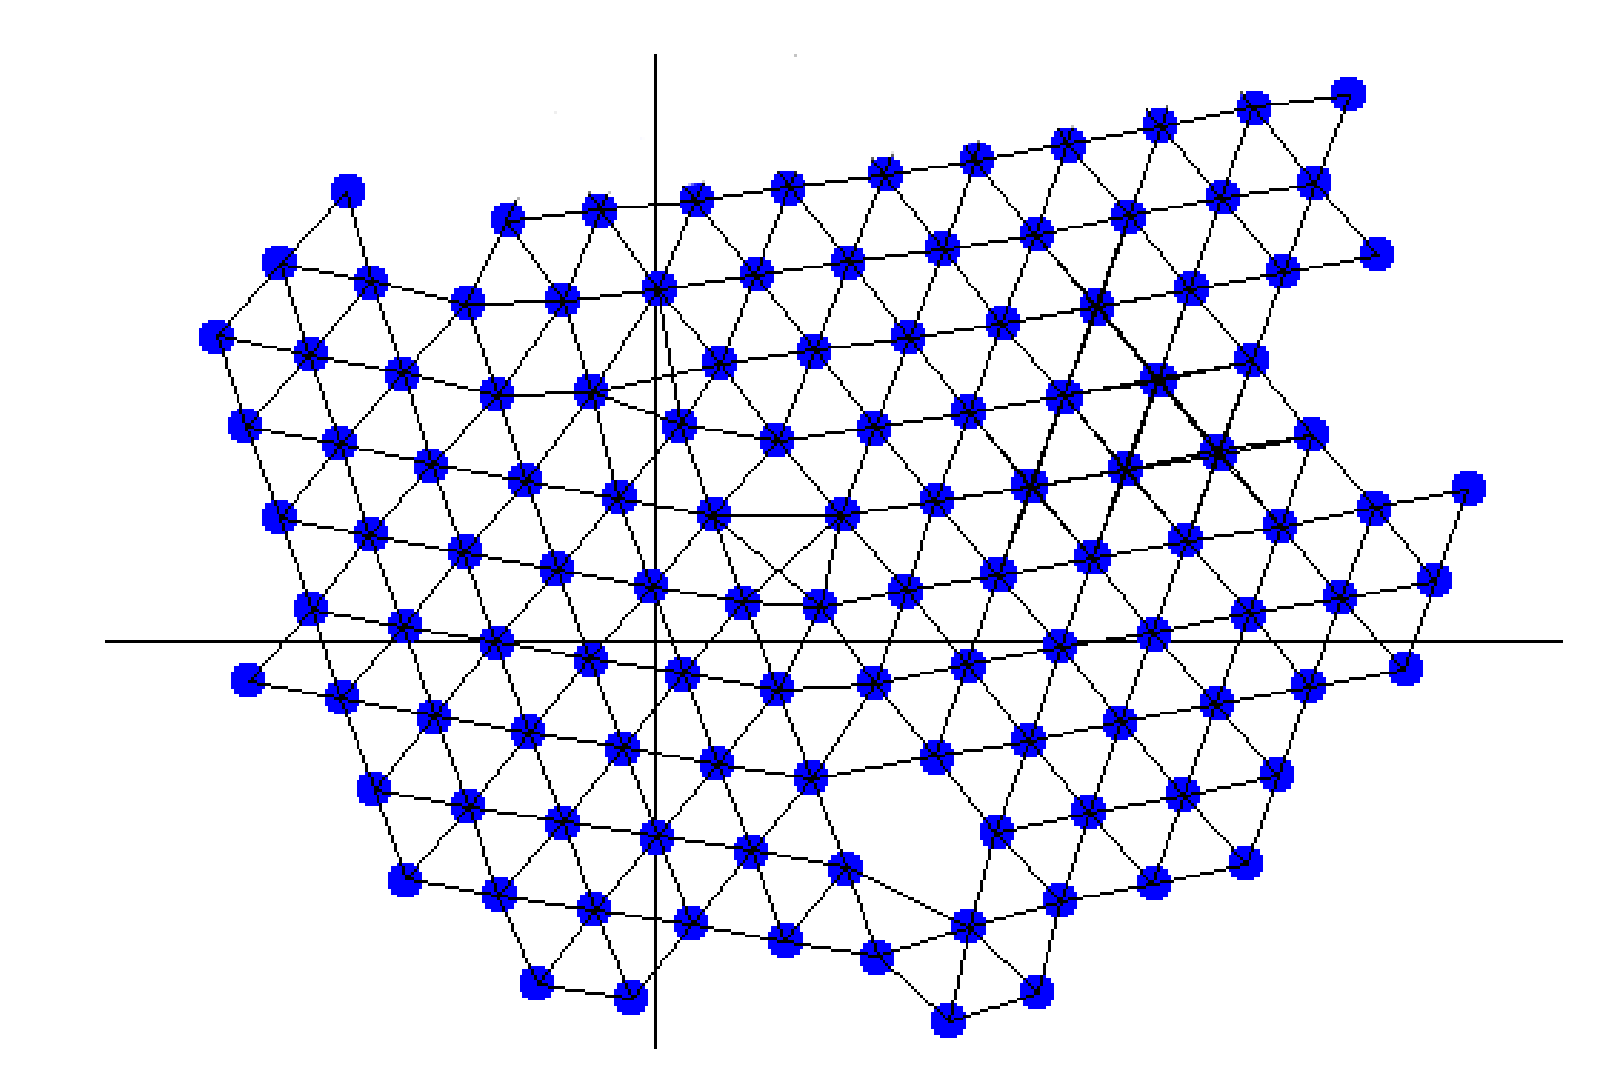
\includegraphics[height=1in]{figs/navarro.png}
      \end{figure}      
    \end{column}
  \end{columns}
  \vspace{3mm}
  \begin{columns}[T] 
    \begin{column}{.45\textwidth}
      \begin{figure}
        \centering
        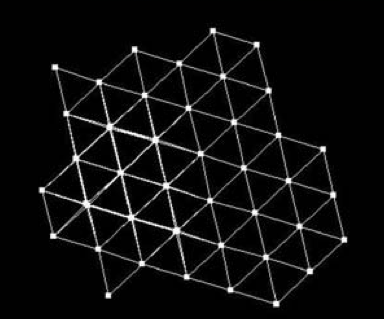
\includegraphics[height=1in]{figs/spears2.png}     
      \end{figure}  
    \end{column}%
    \begin{column}{.45\textwidth}
      \scriptsize{S. Prabhu, W. Li, J. McLurkin, 2012}
      \begin{figure}
        \centering
        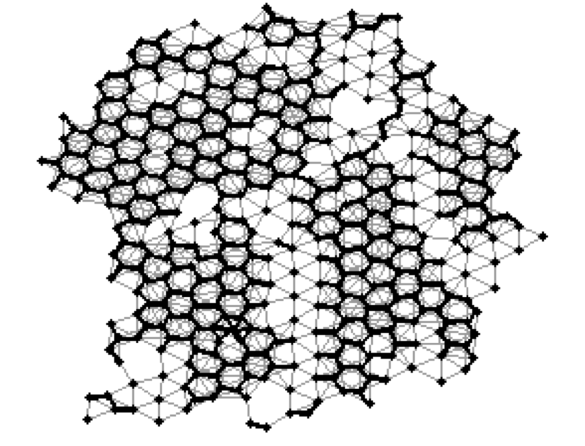
\includegraphics[height=1in]{figs/james.png}
      \end{figure}
    \end{column}
  \end{columns}
\end{frame}

\begin{frame}{Motivation}{}
  \textbf{Question: How to use one algorithm to generate
      various (repeating) lattice pattern formations?}
    \begin{columns}
    \begin{column}{.45\textwidth}
      \begin{figure}
        \centering
        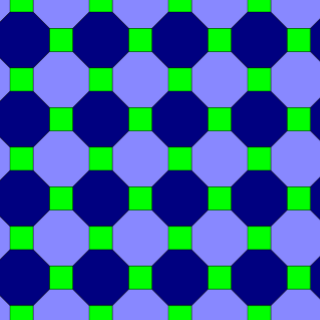
\includegraphics[height=1.5in]{figs/tessellation2}
      \end{figure}
    \end{column}
    \begin{column}{.45\textwidth}
       \begin{figure}
         \centering
        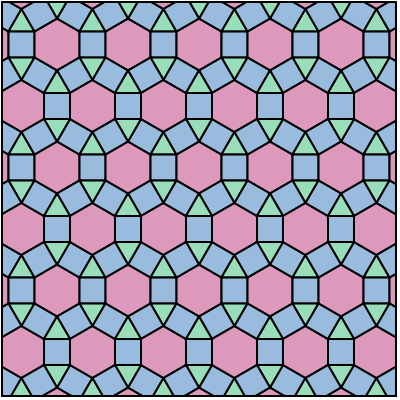
\includegraphics[height=1.5in]{figs/tessellation1}
      \end{figure}
    \end{column}
  \end{columns} 
\end{frame}

\begin{frame}{Simulations}
  \begin{columns}
    \begin{column}{.45\textwidth}
      30 robots, form octagon-square pattern
       \begin{center}
         \includemovie[toolbar,poster,autoplay]{5cm}{5cm}{videos/octsq.mp4}
       \end{center}
    \end{column}
    \begin{column}{.45\textwidth}
      30 robots, form triangle-hexagon-square pattern
       \begin{center}
         \includemovie[toolbar,poster,autoplay]{5cm}{5cm}{videos/trihexsq.mp4}
       \end{center}
     \end{column}
  \end{columns}
\end{frame}

%%%%%%%%%%%%%%%%
\begin{frame}{Robot Model}{}
  \begin{columns}[T] % align columns
    \begin{column}{.55\textwidth}
      \begin{itemize}
      \item Differential Drive robots
      \item Each robot has a unique \textbf{ID}
      \item Use a vector $p = [x, y,
        \theta]^T$ to represent robot's \textbf{pose}
      \item Each robot has a \textbf{range} within which it can
        sense and communicate with other robots
      \item Each robot gets \textbf{observation} of its neighbors'
        IDs and relative poses in its body frame
      \end{itemize}
    \end{column}%
    % right column
    \begin{column}{.45\textwidth}
      \begin{figure}
        \centering
        \begin{tikzpicture}[scale=0.55]
          \draw[dotted, violet, fill=violet!10] (3, 3) circle (3.2);
          \draw[fill=red] (3,3) -- (2.75,3) -- (3.25,3.25) -- (3,2.75) -- cycle;
          \node[color=red] at (3, 2.3) {$r_i$};           
          \draw[fill=blue!50] (0.5,4.5) -- (0.33,4) -- (0.5,4.125) -- (0.67,4)-- cycle;
          \draw[fill=blue!50] (4,5) -- (3.75,5.5) -- (3.75,5.25) -- (3.5,5.25)-- cycle;
          \draw[fill=blue!50] (1,1.5) -- (1.25,1) -- (1.25,1.25) -- (1.5,1.25)-- cycle;
          \draw[fill=blue!50] (5,2.92) -- (4.5,2.75) -- (5,2.58) -- (4.875,2.75)-- cycle;
          \draw[fill=green!50] (-0.5,0.5) -- (-0.5,0.75) -- (-0.75,0.25) -- (-0.25,0.5) -- cycle;
        \end{tikzpicture}
      \end{figure}
      \begin{center}
        Robot $r_i$ has 4 neighbors
      \end{center}
    \end{column}%
  \end{columns}
\end{frame}
%%%%%%%%%%%%%%%%%%%%%%%%%%%%%%%%%%%%%%%%%%%%%%%%%%%%%%%%
\subsection[Lattice Graph]{Lattice Graph}
% definition of lattice graph
\begin{frame}{Input: Lattice Graph}
  \begin{definition}
    A \textbf{lattice graph} is a strongly connected directed
      multigraph in which each edge $e$ is labeled with a rigid body
      transformation $T(e)$ and each $\edge{v}{T(e)}{w}$ has an
      inverse edge $\edge{w}{T(e)^{-1}}{v}$.  
    \end{definition}
    \begin{columns}[T] % align columns
      \begin{column}{.45\textwidth}
        \begin{figure}
          \centering
          \begin{tikzpicture}[->,>=stealth',shorten >=5pt,auto,node distance=1cm]
            \tikzstyle{every state}=[fill=blue,draw=none, text=white]
            \node[state, scale=0.6] (A)         {$0$};
            \path (A) edge [loop above] node {\footnotesize{Tr(0, 40)}} (A)
                      edge [loop left]  node {\footnotesize{Tr(-40,0)}} (A)
                      edge [loop below] node {\footnotesize{Tr(0, -40)}} (A)
                      edge [loop right] node {\footnotesize{Tr(40, 0)}} (A);
          \end{tikzpicture}
        \end{figure}
      \end{column}%
      \begin{column}{.45\textwidth}
        \begin{figure}
          \centering
          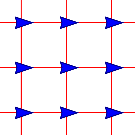
\includegraphics[scale=1]{figs/squarelattice}
        \end{figure}
      \end{column}%
    \end{columns}
\end{frame}


\begin{frame}{Self-Consistent Lattice Graph}
  \begin{definition}
    \small{Given a range $\phi > 0$, call a lattice graph
      \textit{self-consistent} for this range if, for any two paths with the
      same starting node,
      $$\lgpath{v}{T(e_v^{k})}{T(e_m^{w})}{w}, \text{ and }\lgpath{v}{T(e_v^{j})}{T(e_n^{u})}{u},$$
      for which the distance between two ending nodes is less than or equal to
      $\phi$, there exist edges between $w$ and $u$ with right transformation.}
  \end{definition}
  \begin{columns}[T] % align columns
    \begin{column}{.45\textwidth}
      \begin{figure}
        \centering
        \begin{tikzpicture}
          \tikzstyle{every state}=[fill=red!50, draw=none]
          \node[state, scale=0.7] (A) at (2.5,0)  {\large{$v$}};
          \node[state, scale=0.7] (C) at (0, 0.75) {\large{$w$}};
          \node[state, scale=0.7] (D) at (0, -0.75) {\large{$u$}};
          \draw[arc] (A) to[out=150, in=0] (C);
          \draw[arc] (A) to[out=-150,in=0] (D);
          \draw[arc] (C) to[out=-30, in=170] (A);
          \draw[arc] (D) to[out=30, in=-170] (A);
          \node[] at (1, -1.2) {\scriptsize{$\left(0, l, 0\right)$}};
          \node[] at (1, 1.2) {\scriptsize{$\left(\dfrac{l}{2}, l, 0\right)$}};
          % \node[] at (-0.5, 0) {\scriptsize{$(\dfrac{\range}{2}, 0, 0)$}};
        \end{tikzpicture}
      \end{figure}
    \end{column}%
    \begin{column}{.45\textwidth}
      \begin{figure}
        \centering
        \begin{tikzpicture}
          \tikzstyle{every state}=[fill=red!50, draw=none]
          \node[state, scale=0.7] (A) at (2.5,0)   {\large{$v$}};
          \node[state, scale=0.7] (C) at (0, 0.75) {\large{$w$}};
          \node[state, scale=0.7] (D) at (0, -0.75) {\large{$u$}};
          \draw[arc] (A) to[out=150, in=0] (C);
          \draw[arc] (A) to[out=-150,in=0] (D);
          \draw[arc] (C) to[out=-30, in=170] (A);
          \draw[arc] (D) to[out=30, in=-170] (A);
          \draw[arc] (C) to[out=-60, in=60] (D);
          \draw[arc] (D) to[out=120, in=-120] (C);
          \node[] at (1, -1.2) {\scriptsize{$\left(0, l, 0\right)$}};
          \node[] at (1, 1.2) {\scriptsize{$\left(\dfrac{l}{2}, l, 0\right)$}};
          \node[] at (-1, 0) {\scriptsize{$\left(\dfrac{l}{2}, 0, 0\right)$}};
        \end{tikzpicture}
        % \caption{A lattice graph that is self-consistent when $\phi > l$.}
      \end{figure}
    \end{column}%
  \end{columns}
\end{frame}

\begin{frame}{Simulation Example}{Square formation with 10 robots}
  \begin{center}
  \includemovie[toolbar, poster, autoplay]{6cm}{6cm}{videos/square10.mp4}
  \end{center}
\end{frame}

\begin{frame}{Role Function}
  \begin{definition}
    \small{Given a lattice graph $G=(V, E)$ and a set of robots $R = \{
    r_1, \ldots, r_n \}$, $R$ \textbf{satisfies} $G$ if
    there exists a role function $f: R \rightarrow V$ that preserves
    the neighborhood structure of $G$.
    \\
    Specifically, for any $i$ and $j$, if $r_i$ and $r_j$ are neighbors, 
    there must exist an edge
    $e_{ij}: \edge{f(r_i)}{}{f(r_j)}$ in $E$, such that
    $ T(r_j) = T(r_i) T(e_{ij})$.}
  \end{definition}
  \begin{columns}[T] 
    \begin{column}{.4\textwidth}
      \begin{figure}
        \centering
        \begin{tikzpicture}[->,>=stealth',shorten >=5pt,auto,node
          distance=1cm]
            \tikzstyle{every state}=[fill=myred, draw=none, text=white]
            \node[state, scale=0.6] (A) at (0,0)    {$0$};
            \node[state, scale=0.6, fill=mycyan] (B) at (3,0)  {$1$};
            \path (A) edge [bend left=10] node {\scriptsize{Tr(0, 40)}} (B)
                  (A) edge [bend left=45] node {\scriptsize{Tr(-35,-20)}} (B)
                  (A) edge [bend left=90] node
                  {\scriptsize{Tr(35,-20)}} (B)
                  (B) edge [bend left=10]  node {\scriptsize{Tr(-40,0)}} (A)
                  (B) edge [bend left=45]  node
                  {\scriptsize{Tr(35,20)}} (A)
                  (B) edge [bend left=90]  node {\scriptsize{Tr(-35,20)}} (A);
        \end{tikzpicture}
      \end{figure}
    \end{column}%
    \begin{column}{.5\textwidth}
      \begin{figure}
        \centering
        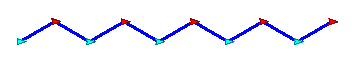
\includegraphics[width=0.75\linewidth]{figs/bad-hexagon}
      \end{figure}
      \begin{figure}
        \centering
        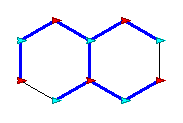
\includegraphics[scale=0.8]{figs/good-hexagon}
        \end{figure}
    \end{column}%
  \end{columns}
\end{frame}

\begin{frame}{Evaluation Criteria}
  \begin{itemize}
  \item \textbf{Efficiency}\\
    %\begin{definition}
    A robot $r_i$ is \textbf{static} at time $t$ if its pose $p_i$
    remains the same at all future times, so that 
    $$p_i(t') = p_i(t) \quad \mbox {for all } t' > t$$    
  %\end{definition}
  Define the \textbf{execution time} $\bar{t}$ of the system as the smallest time
  when all the robots reach in static states
  \item \textbf{Quality} \\
    When all robots reach static positions, for a robot $r_i$
    with $N_i$ neighbors and $E_i$ outgoing edges from its role vertex. 
    Define a non-fulfillment ratio:
    $$\Gamma = \dfrac{1}{n}\sum\limits_{i=1}^n \frac{E_i - N_i}{E_i}$$
    to measure the overall lattice quality
  \end{itemize}
  
\end{frame}
%%%%%%%%%%%%%%%%%%%%%%%%%%%%%%%%%%%%%%%%%%%%%%%%%%%%%%%%
\subsection[Algorithm]{Algorithm}
\begin{frame}{Algorithm}
  \textbf{General Description}
  \begin{columns}[T] % align columns
   \begin{column}{.45\textwidth}
     Robot broadcasts message containing its
     \begin{itemize}
     \item \textcolor{red}{authority} 
     \item \textcolor{red}{matching}
     \item \textcolor{red}{opening}
     \end{itemize}

     \begin{enumerate}
     \item Form tree structure
     \item Select roles
     \item Use tree structure to compute local task assignment
     \item Make movement decision
     \end{enumerate}
    \end{column}%
    \begin{column}{.45\textwidth}
      \begin{animateinline}[
  begin={%
    \begin{tikzpicture}%
      [post/.style={->,>=stealth', semithick, draw=blue!50},
      node/.style={circle,fill=red!20,draw,font=\sffamily\small}]%
      \useasboundingbox (0,0) rectangle (5,5);
    },
    end={\end{tikzpicture}}
  ]{10}
  \draw[fill=blue!50] (3,3) -- (2.75,3) -- (3.25,3.25) -- (3,2.75)  -- cycle;
  \draw[fill=blue!50] (0.5,4.5) -- (0.33,4) -- (0.5,4.125) -- (0.67,4) -- cycle;
  \draw[fill=blue!50] (1,1.5) -- (1.25,1) -- (1.25,1.25) --
  (1.5,1.25) -- cycle;
  \newframe*
  \multiframe{10}{rP = 0.1 +.1}{ 
    \draw[fill=blue!50] (3,3) -- (2.75,3) -- (3.25,3.25) -- (3,2.75)  -- cycle;
    \node[color=black] at (3, 4.5) {broadcast Message};           
    \draw[fill=blue!50] (0.5,4.5) -- (0.33,4) -- (0.5,4.125) -- (0.67,4) -- cycle;
    \draw[fill=blue!50] (1,1.5) -- (1.25,1) -- (1.25,1.25) --
    (1.5,1.25) -- cycle;
    \path (3,3) -- (1.25, 1.25) node[pos=\rP] (q){};
    \draw[post] (3,3) -- (q.west);
    
    \path (3,3) -- (0.5, 4.125) node[pos=\rP] (q){};
    \draw[post] (3,3) -- (q.west);
    
    \path (1.5, 1.25) -- (3,2.5) node[pos=\rP] (q){};
    \draw[post] (1.5, 1.25) -- (q.west);
    
    \path (1.25, 1.5) -- (0.5, 4.125) node[pos=\rP] (q){};
    \draw[post] (1.25, 1.5) -- (q.south);
    
    \path (0.5, 4.5) -- (3.25, 3.25) node[pos=\rP] (q){};
    \draw[post] (0.5, 4.5) -- (q.north);

    \path (0.33, 4) -- (1, 1.5) node[pos=\rP] (q){};
    \draw[post] (0.33, 4) -- (q.north);
  }
  \newframe*
  \multiframe{10}{rP = 0.1 +.1}{ 
    \draw[fill=red] (3,3) -- (2.75,3) -- (3.25,3.25) -- (3,2.75)  -- cycle;
    \node[color=red] at (3, 2.3) {$root$};           
    \draw[fill=blue] (0.5,4.5) -- (0.33,4) -- (0.5,4.125) --
    (0.67,4) 	-- cycle;
    \node[color=blue] at (1, 3.75) {$descendant$};           
    \draw[fill=blue] (1,1.5) -- (1.25,1) -- (1.25,1.25) -- (1.5,1.25)  -- cycle;
    \node[color=blue] at (2.5,1.5) {$descendant$};
    \node[color=black] at (3, 4.5) {Form Tree Structure};
    \path (3,3) -- (1.25, 1.25) node[pos=\rP] (q){};
    \draw[post, color=red] (3,3) -- (q);
    
    \path (3,3) -- (0.5, 4.125) node[pos=\rP] (q){};
    \draw[post, color=red] (3,3) -- (q);
  }
  \newframe*
  \multiframe{10}{rP = 0.1 +.1}{ 
    \draw[fill=red] (3,3) -- (2.75,3) -- (3.25,3.25) -- (3,2.75)  -- cycle;
    \draw[fill=blue] (0.5,4.5) -- (0.33,4) -- (0.5,4.125) --
    (0.67,4) 	-- cycle;
    \draw[fill=blue] (1,1.5) -- (1.25,1) -- (1.25,1.25) -- (1.5,1.25)  -- cycle;
    \node[color=black] at (3, 4.5) {Assign Task};  
    % \path (3,3) -- (1.25, 1.25) node[pos=\rP] (q){};
    \draw[post, color=red] (3,3) -- (1.25, 1.25);
    % \path (3,3) -- (0.5, 4.125) node[pos=\rP] (q){};
    \draw[post, color=red] (3,3) -- (0.5,4.125);
    \draw[red, dotted] (1,3) -- (0.75,3) -- (1.25,3.25) -- (1,2.75) -- cycle;
    \draw[red, dotted] (3,1) -- (2.75,1) -- (3.25,1.25) -- (3,0.75) -- cycle;
    \draw[dashed](1.25,1.25) -- (3,1);
    \draw[dashed](0.5,4.125) -- (1,3);
  }
  \newframe*
  \multiframe{10}{rP = 0.1 +.1}{ 
    \draw[fill=red] (3,3) -- (2.75,3) -- (3.25,3.25) -- (3,2.75)  -- cycle;
    \node[color=black] at (3, 4.5) {Movement Control};  
    \draw[post, color=red] (3,3) -- (1,3);
    \draw[post, color=red] (3,3) -- (3,1);
    \draw[fill=blue] (1,3) -- (0.75,3) -- (1.25,3.25) -- (1,2.75) -- cycle;
    \draw[fill=blue] (3,1) -- (2.75,1) -- (3.25,1.25) -- (3,0.75) -- cycle;
  }
\end{animateinline}
    \end{column}%
  \end{columns}
\end{frame}
%%%%%%%%%%%%%%%%
\subsubsection[Algorithm: Authority]{Authority Tree}
\begin{frame}{Authority}
  \textbf{Define authority and comparison operator}
  \begin{definition}
    \small{An \textbf{authority} is an ordered list of robot IDs
      $$(\id_1, \ldots, \id_k)$$
      The first ID in the list, $\id_1$ is called the \textbf{root} ID.
      The final ID in the list, $\id_k$ is called the \textbf{sender} ID.}
  \end{definition}
  \begin{definition}
    \small{Authority $A_2$ is \textbf{higher than} $A_1$ if:}
    \begin{itemize}
    \item \small{root ID of $A_2 >$ root ID of $A_1$, or}
    \item \small{length of $A_2 <$  length of $A_1$ if they have the same root, or}
    \item \small{sender ID of $A_2 >$ sender ID of $A_1$ if they have the same root and length}
    \end{itemize}
  \end{definition}
\end{frame}
%%%%%%%%%%%%%%%%
\begin{frame}{1.Construct Authority Tree}{Decide to be root or descendant}
  \textbf{Key Idea:} Each robot forms an authority containing only its own ID,
  compares it with the authorities of remaining messages. The robots use these
  authorities to establish a collection of authority trees
  \begin{columns}[T] % align columns
    \begin{column}{.45\textwidth}
      \begin{itemize}
      \item {\textcolor{red}{Root}: Robot who has the highest authority}
      \item {\textcolor{blue}{Descendant}: Robot selects the neighbor who sends
          the highest authority and has matching with it as its parent}
      \item {\textcolor{orange}{Orphan}: Robot who has no parent}
      \end{itemize}     
    \end{column}%
    \begin{column}{.5\textwidth}
       \begin{animateinline}[
  begin={%
    \begin{tikzpicture}%
      [post/.style={->,>=stealth', thick, draw=blue!50},
      node/.style={circle,fill=red!20,draw,font=\sffamily\small}]%
      \useasboundingbox (0,1) rectangle (5,5);
    },
    end={\end{tikzpicture}}
  ]{10}
  \draw[fill=red] (2,5) -- (1.83,4.5) -- (2,4.625) --
  (2.17,4.5) -- cycle;
  \node[color=red] at (1.5, 4.7) {$(1)$};
  \draw[dashed, red] (3, 4) circle (3);
  % center is (3,4)
  \draw[fill=red] (3,4) -- (2.75,4) -- (3.25,4.25) -- (3,3.75)  -- cycle;
  \node[color=red] at (2.75, 3.5) {$(2)$};
  % center is (0.5, 4.5)
  \draw[dashed, red] (0.5,4.5) circle (2.8);
  \draw[fill=red] (0.5,4.5) -- (0.33,4) -- (0.5,4.125) --
  (0.67,4) -- cycle;
  \node[color=red] at (0.5, 3.75) {$(4)$};
  % center is (3.75,2)
  \draw[dashed, red] (3.75,2) circle (2.5);
  \draw[fill=red] (3.5,2.5) -- (3.75,2) -- (3.75,2.25) --
  (4,2.25) -- cycle;
  \node[color=red] at (3.3, 2) {$(3)$};
  %%%% 
  \newframe*
  \multiframe{10}{rP= 0.1+ .1, r = 1 + 1}{
    \draw[fill=orange] (2,5) -- (1.83,4.5) -- (2,4.625) --
    (2.17,4.5) -- cycle;
    \node[color=orange] at (1.5, 4.7) {$(1)$};
    \draw[dashed, blue] (3, 4) circle (2.8);
    % center is (3,4)
    \draw[fill=blue] (3,4) -- (2.75,4) -- (3.25,4.25) --
    (3,3.75)  -- cycle;
    \node[color=blue] at (2.75, 3.5) {$(4,2)$};
    % center is (0.5, 4.5)
    \draw[dashed, red] (0.5,4.5) circle (2.8);
    \draw[fill=red] (0.5,4.5) -- (0.33,4) -- (0.5,4.125) --
    (0.67,4) -- cycle;
    \node[color=red] at (0.5, 3.75) {$(4)$};
    % center is (3.75,2)
    \draw[dashed, red] (3.75,2) circle (2.8);
    \draw[fill=red] (3.5,2.5) -- (3.75,2) -- (3.75,2.25) --
    (4,2.25) -- cycle;
    \node[color=red] at (3.3, 2) {$(3)$};
    \path (0.5,4.125) -- (3,4) node[pos=\rP] (q){};
    \draw[post] (0.5,4.125) -- (q);
  }
  \newframe*
  \multiframe{10}{r = 1 + 1}{ 
    \draw[fill=orange] (2,5) -- (1.83,4.5) -- (2,4.625) --
    (2.17,4.5) -- cycle;
    \node[color=orange] at (1.5, 4.7) {$(1)$};
    \draw[dashed, blue] (3, 4) circle (2.8);
    % center is (3,4)
    \draw[fill=blue] (3,4) -- (2.75,4) -- (3.25,4.25) --
    (3,3.75)  -- cycle;
    \node[color=blue] at (2.75, 3.5) {$(4,2)$};
    % center is (0.5, 4.5)
    \draw[dashed, red] (0.5,4.5) circle (2.8);
    \draw[fill=red] (0.5,4.5) -- (0.33,4) -- (0.5,4.125) --
    (0.67,4) -- cycle;
    \node[color=red] at (0.5, 3.75) {$(4)$};
    % center is (3.75,2)
    \draw[dashed, blue] (3.75,2) circle (2.8);
    \draw[fill=blue] (3.5,2.5) -- (3.75,2) -- (3.75,2.25) --
    (4,2.25) -- cycle;
    \node[color=blue] at (3, 2) {$(4,2,3)$};
    \draw[post] (0.5,4.125) -- (2.87,4);
  }
  \newframe*
  \multiframe{10}{rP = 0.1 +.1, r = 1 + 1}{ 
    \draw[fill=orange] (2,5) -- (1.83,4.5) -- (2,4.625) --
    (2.17,4.5) -- cycle;
    \node[color=orange] at (1.5, 4.7) {$(1)$};
    \draw[dashed, blue] (3, 4) circle (2.8);
    % center is (3,4)
    \draw[fill=blue] (3,4) -- (2.75,4) -- (3.25,4.25) --
    (3,3.75)  -- cycle;
    \node[color=blue] at (2.75, 3.5) {$(4,2)$};
    % center is (0.5, 4.5)
    \draw[dashed, red] (0.5,4.5) circle (2.8);
    \draw[fill=red] (0.5,4.5) -- (0.33,4) -- (0.5,4.125) --
    (0.67,4) -- cycle;
    \node[color=red] at (0.5, 3.75) {$(4)$};
    % center is (3.75,2.25)
    \draw[dashed, blue] (3.75,2) circle (2.8);
    \draw[fill=blue] (3.5,2.5) -- (3.75,2) -- (3.75,2.25) --
    (4,2.25) -- cycle;
    \node[color=blue] at (3, 2) {$(4,2,3)$};
    \draw[post] (0.5,4.125) -- (2.87,4);

    \path (3,4) -- (3.75, 2.25) node[pos=\rP] (q){};
    \draw[post] (3,4) -- (q);        
  }
\end{animateinline}
    \end{column}
  \end{columns}
\end{frame}
%%%%%%%%%%%%%%%%
\begin{frame}{Combined Communication-Authority Graph}
  \begin{definition}
    \small{Given a set of robots $R =\{r_1, ..., r_n\}$, the \textbf{communication
        graph} is a graph in which each vertex is a robot, and there exists an
      undirected edge between two vertices if corresponding robots are
      neighbors.}
  \end{definition}
  \begin{definition}
    \small{The \textbf{authority graph} is a graph in which each vertex is a
      robot, and there exists an directed edge to each descendant robot to its
      parent.}
  \end{definition}
  \begin{columns}
    \begin{column}{0.5\textwidth}
      \small{A combined communication-authority graph $\G$ contains:
        \begin{enumerate}
        \item Directed edges, labeled $I$, indicate parent-child relationships
        \item Undirected edges, labeled $II$, belong to the communication graph
          but not the authority graph
        \end{enumerate}
      }
    \end{column}
    \begin{column}{0.4\textwidth}
      \begin{figure}
  \centering
  %\begin{minipage}[b]{0.45\linewidth}
  \begin{tikzpicture}
    \tikzstyle{every state}=[fill=red, draw=none]
    \node[state, scale=0.5] (A) at (1,0)    {$3$};
    \node[state, scale=0.5, fill=orange] (B) at (2.5,0)  {$0$};
    \node[state, scale=0.5, fill=cyan] (C) at (0, 1) {$1$};
    \node[state, scale=0.5, fill=cyan] (D) at (0, -1) {$2$};
    \draw[edge] (A) -- (C);
    \draw[edge] (A) -- (D);
    \draw[dashed] (C) -- (D);
    \draw[dashed] (A) -- (B);
    \node[] at (1.75, 0.3) {\footnotesize{$II$}};
    \node[] at (-0.5, 0) {\footnotesize{$II$}};
    \node[] at (0.75, 0.5) {\footnotesize{$I$}};
    \node[] at (0.75, -0.5) {\footnotesize{$I$}};
  \end{tikzpicture}
  % \end{minipage}
  % \begin{minipage}[b]{0.45\linewidth}
  %   \begin{tikzpicture}
  %     \node[] (A) at (1,0)    {\footnotesize{$\langle3\rangle$}};
  %     \node[] (B) at (2.5,0)  {\footnotesize{$\langle0\rangle$}};
  %     \node[] (C) at (0, 1)   {\footnotesize{$\langle3,1\rangle$}};
  %     \node[] (D) at (0, -1)  {\footnotesize{$\langle3,2\rangle$}};
  %     \draw[edge] (A) -- (C);
  %     \draw[edge] (A) -- (D);
  %   \end{tikzpicture}
  % \end{minipage}
  %\caption{}
\end{figure}
    \end{column}
  \end{columns}
\end{frame}
%%%%%%%%%%%%%%%%
\begin{frame}{Neighborhood Property}
  \begin{definition}
    \small{Define the \textbf{neighborhood properties} of a robot as:\\
      (1) the ID of its parent,\\
      (2) the number of its children, and\\
      (3) the lowest ID of its children.}
  \end{definition}
  \begin{definition}
    \small {The \textbf{pivot robot} is the robot with the highest authority in
      $\G\two$ for which the neighborhood properties differ from its
      neighborhood properties in $\G\one$.}
  \end{definition}
  \begin{figure}
  \centering
  \begin{minipage}[b]{0.45\linewidth}
    \begin{tikzpicture}[scale=0.75]
      \tikzstyle{every state}=[draw=none]
      \node[state, scale=0.5, fill=red]  (A) at (1,0)    {$3$};
      \node[state, scale=0.5, fill=cyan] (B) at (2.5,0)  {$0$};
      \node[state, scale=0.5, fill=cyan] (C) at (0, 1)   {$1$};
      \node[state, scale=0.5, fill=cyan] (D) at (0, -1)  {$2$};
      \draw[dashed] (A) -- (C);
      \draw[edge] (A) -- (D);
      \draw[edge] (D) -- (C);
      \draw[edge] (A) -- (B);
      \node[color=black] at (2, 1) {$\G\one$};
    \end{tikzpicture}
  \end{minipage}
  \begin{minipage}[b]{0.45\linewidth}
    \begin{tikzpicture}[scale=0.75]
      \tikzstyle{every state}=[fill=red, draw=none]
      \node[state, scale=0.5] (A) at (1,0)    {$3$};
      \node[state, scale=0.5, fill=orange] (B) at (2.5,0)  {$0$};
      \node[state, scale=0.5, fill=cyan] (C) at (0, 1) {$1$};
      \node[state, scale=0.5, fill=cyan] (D) at (0, -1) {$2$};
      \draw[edge] (A) -- (C);
      \draw[edge] (A) -- (D);
      \draw[dashed] (C) -- (D);
      \draw[dashed] (A) -- (B);
      \node[color=black] at (2, 1) {$\G\two$};
    \end{tikzpicture}
  \end{minipage}
  \caption{\scriptsize{Robot $3$ is the pivot robot. The neighborhood properties
      of robot $3$ are $(3,2,0)$ and $(3,2,1)$.}}
\end{figure}  
\end{frame}

\begin{frame}{Progress of Proof}{Total order over communication-authority graph}
Define a total order to compare two connected combined communication and
authority graphs $\G\one$ and $\G\two$ formed by the same set of robots,
denoted as $\leq$.
\begin{block}{Total Order}
\small{
  $\G\one \leq \G\two$ if for the pivot robot:
  \begin{enumerate}
  \item the parent-ID in $\G\two$ is greater than the parent-ID in $\G\one$,
    otherwise,
  \item the children number in $\G\two$ is greater than the
    children number in $\G\one$, otherwise,
  \item the lowest child-ID in $\G\two$ is greater than the
    lowest child-ID in $\G\one$.
  \end{enumerate}}
\end{block}
\begin{figure}
  \centering
  \begin{minipage}[b]{0.45\linewidth}
    \begin{tikzpicture}
      \tikzstyle{every state}=[draw=none]
      \node[state, scale=0.5, fill=cyan] (A) at (1,0)     {$3$};
      \node[state, scale=0.5, fill=orange] (B) at (2.5,0) {$0$};
      \node[state, scale=0.5, fill=red] (C) at (0,1)      {$1$};
      \draw[edge] (A) -- (C);
      \draw[dashed] (A) -- (B);
      \node[color=black] at (2,1) {$\G\one$};
    \end{tikzpicture}
  \end{minipage}
  \begin{minipage}[b]{0.45\linewidth}
    \begin{tikzpicture}
      \tikzstyle{every state}=[draw=none]
      \node[state, scale=0.5, fill=red] (A) at (1,0)    {$1$};
      \node[state, scale=0.5, fill=cyan] (B) at (2.5,0) {$3$};
      \node[state, scale=0.5, fill=cyan] (C) at (0,1)   {$0$};
      \draw[edge] (B) -- (A);
      \draw[edge] (A) -- (C);
      \node[color=black] at (2,1) {$\G\two$};
    \end{tikzpicture}
  
  \end{minipage}
\end{figure}
 \textcolor{scred}{\footnotesize{Intuition: prove the combined
      communication and authority graph eventually becomes stable.}}
\end{frame}

%%%%%%%%%%%%%%%%
\subsubsection[Algorithm: Task Assignment]{Task Assignment}
\begin{frame}{Matching}{}
  \begin{definition}    
    \small{A \textbf{matching} for a robot is a function $\eta : \{\id(r_a),
      \id(r_b), \ldots \} \rightarrow \{\emptyset,e_{u}^v, e_{u}^w,
      \ldots\} $ that associates each neighbor ID with either a lattice
      graph edge from its role vertex or with the null value
      $\emptyset$.}
  \end{definition}
  \begin{center}
    \definecolor{myblue}{RGB}{56,94,141}
\newcommand\xsetpos{6}

\begin{tikzpicture}[scale=.4,
                    arrow/.style={thick,->,myblue},
                    set name/.style={font=\color{myblue}\Large\bfseries\sf},
                    set/.style={thick,myblue},
                    every node/.style={circle},
                    font=\sf
                    ]
\draw[set] (0,0) circle [x radius=1.5cm, y radius=5cm]
           (\xsetpos,0) circle [x radius=1.5cm, y radius=5cm];

\node[set name] at (0,-6) {\footnotesize{Neighbor ID}};
\node[set name] at (\xsetpos,-6) {\footnotesize{Edge}};  

\node (a1) at (0,3)  {\footnotesize{$\id(r_a)$}};
\node (a2) at (0,1)  {\footnotesize{$\id(r_b)$}};
\node (a3) at (0,0) {\footnotesize{$\vdots$}};
\node (a4) at (0,-2) {\footnotesize{$\id(r_c)$}};
\node (a5) at (0,-3) {\footnotesize{$\id(r_d)$}};

\node (b1) at (\xsetpos,3)  {\footnotesize{$e_u^v$}};
\node (b2) at (\xsetpos,1)  {\footnotesize{$e_u^w$}};
\node (b3) at (\xsetpos,0) {\footnotesize{$\vdots$}}; 
\node (b4) at (\xsetpos,-2) {\footnotesize{$\emptyset$}};
\begin{scope}[arrow]
  \draw (a1.east) -- (b2);
  \draw (a2.east) -- (b1);
  %\draw (a3.east) -- (b3);
  \draw (a4.east) -- (b4); 
  \draw (a5.east) -- (b4);
\end{scope}

\end{tikzpicture}    
  \end{center}
\end{frame}

\begin{frame}{2. Local Task Assignment}{Hungarain Algorithm}
  To compute an optimal matching of a robot with $N$ neighbors and $E$
  out-going edges of its role in the lattice graph, define a weight
  matrix of size $\min(N,E) \times E$ and apply
  \textcolor{scred}{Hungarian Algorithm} (Harold W. Kuhn, 1955).
    \begin{columns}[T] % align columns
      \begin{column}{.45\textwidth}
        \begin{enumerate}
        \item \small{Each row corresponds to a neighbor}
        \item \small{Each column corresponds to an out-going edge of robot's role}
        \item \small{The entries of the matrix are the Euclidean distance
          between current position of each neighbor and the desired
          position if matched with a lattice graph edge}
        \end{enumerate}
      \end{column}%
      \begin{column}{.45\textwidth}
        \vspace{3mm}
        \begin{animateinline}[
  begin={%
    \begin{tikzpicture}%
      [post/.style={->,>=stealth', thin, draw=blue!50},
      node/.style={circle,fill=red!20,draw,font=\sffamily\small},
      scale=0.8]%
      % \useasboundingbox (0,0) rectangle (5,5);
    },
    end={\end{tikzpicture}}
  ]{10}
  \draw[fill=blue!50] (0.5,4.5) -- (0.33,4) -- (0.5,4.125) -- (0.67,4) -- cycle;
  \draw[fill=blue!50] (4,5) -- (3.75,5.5) -- (3.75,5.25) -- (3.5,5.25) -- cycle;
  \draw[fill=green!50] (1,3.5) -- (1.25,3) -- (1.25,3.25) -- (1.5,3.25) -- cycle;
  \draw[fill=blue!50] (5,2.92) -- (4.5,2.75) -- (5,2.58) -- (4.875,2.75) -- cycle;
  \draw[fill=blue!50] (0,2.5) -- (0,2.75) -- (-0.25,2.25) -- (0.25,2.5) -- cycle;
  
  \draw[color=red] (4,4) -- (3.75,4) -- (4.25,4.25) -- (4,3.75) -- cycle;
  \draw[color=red] (2,2) -- (1.75,2) -- (2.25,2.25) -- (2,1.75) -- cycle;
  \draw[color=red] (2,4) -- (1.75,4) -- (2.25,4.25) -- (2,3.75) -- cycle;
  \draw[color=red] (4,2) -- (3.75,2) -- (4.25,2.25) -- (4,1.75) -- cycle;
  \newframe*
  \multiframe{10}{r = 1 + 1}{ 
    \draw[fill=red] (3,3) -- (2.75,3) -- (3.25,3.25) -- (3,2.75) -- cycle;
    \draw[fill=blue!50] (0.5,4.5) -- (0.33,4) -- (0.5,4.125) -- (0.67,4) -- cycle;
    \draw[fill=blue!50] (4,5) -- (3.75,5.5) -- (3.75,5.25) -- (3.5,5.25) -- cycle;
    \draw[fill=green!50] (1,3.5) -- (1.25,3) -- (1.25,3.25) -- (1.5,3.25) -- cycle;
    \draw[fill=blue!50] (5,2.92) -- (4.5,2.75) -- (5,2.58) -- (4.875,2.75) -- cycle;
    \draw[fill=blue!50] (0,2.5) -- (0,2.75) -- (-0.25,2.25) -- (0.25,2.5) -- cycle;
    
    \draw[color=red] (4,4) -- (3.75,4) -- (4.25,4.25) -- (4,3.75) -- cycle;
    \draw[color=red] (2,2) -- (1.75,2) -- (2.25,2.25) -- (2,1.75) -- cycle;
    \draw[color=red] (2,4) -- (1.75,4) -- (2.25,4.25) -- (2,3.75) -- cycle;
    \draw[color=red] (4,2) -- (3.75,2) -- (4.25,2.25) -- (4,1.75) -- cycle;
    
    \draw[dashed](0.5, 4.25) -- (2,4);
    \draw[dashed](3.75,5.25) -- (4,4);
    \draw[dashed](4.75,2.75) -- (4,2);
    \draw[dashed](0,2.5) -- (2,2);
  }
\end{animateinline}
        \vspace{3mm}
        \begin{flushleft}
          \footnotesize{5 neighbors, 4 out-going edges.}
        \end{flushleft}
      \end{column}%
    \end{columns}
\end{frame}
\begin{frame}{Opening}{}
  \begin{definition}
    \small{An \textbf{opening} is a position where there is no robot and is
    not assigned by a robot yet.}
   \end{definition}
   \begin{columns}[T] % align columns
   \begin{column}{.45\textwidth}
     An opening can be found by a robot:
     \begin{itemize}
     \item \small{locally, if the number of its neighbors is less than its
       out-degree, or}
     \item \small{choosing the nearest position from received messages}
     \end{itemize}
     \begin{figure}
       \centering
       \begin{tikzpicture}[->,>=stealth',shorten >=5pt,auto,node
         distance=1cm]
         \tikzstyle{every state}=[fill=myred, draw=none, text=white]
         \node[state, scale=0.6] (A) at (0,0)    {$0$};
         \path (A) edge [loop left] node {\footnotesize{Tr(40, 0)}} (A)
                   edge [loop right] node {\footnotesize{Tr(-40, 0)}} (A);
       \end{tikzpicture}
       \caption{\footnotesize{Lattice graph representing a single line.}}
     \end{figure}
    \end{column}%
    \begin{column}{.5\textwidth}
      \begin{animateinline}[
  begin={%
    \begin{tikzpicture}%
      [post/.style={->,>=stealth', semithick},
      node/.style={circle,fill=red!20,draw,font=\sffamily\small}]%
      \useasboundingbox (-0.5,-0.5) rectangle (4.5,4.5);
    },
    end={\end{tikzpicture}}
  ]{10}
  \draw[red] (3,3) -- (2.75,3) -- (3.25,3.25) -- (3,2.75)  -- cycle;
  \node[color=black] at (1, 4.7) {local opening};  
  \draw[fill=red] (2,2) -- (1.75,2) -- (2.25,2.25) -- (2,1.75) -- cycle;
  \draw[fill=red] (1,1) -- (0.75,1) -- (1.25,1.25) --
  (1,0.75) -- cycle;
  \draw[red] (0,0) -- (-0.25,0) -- (0.25,0.25) --
  (0,-0.25) -- cycle;
  %\draw[fill=red] (3,2) -- (2.75,2) -- (3.25,2.25) -- (3,1.75) -- cycle;
  \draw[dashed] (3,3) -- (2,2);
  \draw[dashed] (1,1) -- (0,0);   
  \draw[post] (1,1) -- (2,2);
  %\draw[post] (2,2) -- (3,2);
  \node[color=black] at (2, 1.5) {$(10)$};
  \node[color=black] at (1, 0.5) {$(10)$};
  \newframe*
  \multiframe{10}{r = 1 + 1}{
    \draw[fill=red] (3,3) -- (2.75,3) -- (3.25,3.25) -- (3,2.75)  -- cycle;
    \draw[red] (4,4) -- (3.75,4) -- (4.25,4.25) -- (4,3.75)  -- cycle;
    \node[color=black] at (1, 4.7) {local opening};  
    \draw[fill=red!30] (2,2) -- (1.75,2) -- (2.25,2.25) -- (2,1.75) -- cycle;
    \draw[fill=red] (1,1) -- (0.75,1) -- (1.25,1.25) --
    (1,0.75) -- cycle;
    \draw[red] (0,0) -- (-0.25,0) -- (0.25,0.25) --
    (0,-0.25) -- cycle;
    \draw[post] (2,2) -- (3,3);
    \draw[dashed] (1,1) -- (0,0);   
    \draw[post] (1,1) -- (2,2);
    \draw[dashed] (3,3) -- (4,4);
    \node[color=black] at (2, 1.5) {$(20)$};
    \node[color=black] at (1, 0.5) {$(10)$};
    \node[color=black] at (3, 2.5) {$(10)$};
  }
\end{animateinline}
    \end{column}%
  \end{columns}
\end{frame}

\begin{frame}{Example}{Line formation}
  \begin{center}
    \includemovie[toolbar,poster,autoplay]{7cm}{7cm}{videos/line.mp4}
  \end{center}
\end{frame}
%%%%%%%%%%%%%%%%
\subsubsection[Algorithm: Motion]{Motion Strategy}
\begin{frame}{3. Robot Movement Strategy}{}
  \tikzstyle{decision} = [diamond, draw, fill=red!10, 
text width=4em, text badly centered, node distance=3cm, inner sep=0pt]
\tikzstyle{block} = [rectangle, draw, fill=blue!10, 
text width=5em, text centered, rounded corners]%, minimum height=2em]
\tikzstyle{line} = [draw, -latex']

\begin{figure}    
  \centering
  \begin{tikzpicture}
    \node [block] (init) {\footnotesize{Start}};
    \node [decision, below of=init, node distance=2cm] (decide) {\footnotesize{Root?}};
    \node [block, below of=decide, node distance=2cm] (stop) {\footnotesize{Stay}};
    \node [decision, right of=decide, node distance=3.5cm] (decideagain) {\footnotesize{Assigned?}};
    \node [block, right of=decideagain, node distance=3.5cm, text width=6em] (away)
    {\footnotesize{Move towards nearest opening}};
    \node [block, below of=decideagain, node distance=3cm, text width=9em] (go)
    {\footnotesize{Move towards assigned destination}};
    % Draw edges
    \path [line] (init) -- (decide);
    \path [line] (decide) -- node [xshift=-0.5cm]{yes}(stop);
    \path [line] (decide) -- (stop);
    \path [line] (decide) -- node [yshift=0.3cm] {no} (decideagain);
    \path [line] (decideagain) -- node [yshift=0.3cm] {no} (away);
    \path [line] (decideagain) -- node [xshift=-0.5cm] {yes} (go);
  \end{tikzpicture}
\end{figure}
\end{frame}
%%%%%%%%%%%%%%%%
\begin{frame}{Bounded Movement}{}
  \textbf{Goal: Keep descendant stay in the range of its parent}
    \begin{columns}[T] % align columns
      \begin{column}{.5\textwidth}
        \begin{itemize}
        \item \small{Descendant can reach anywhere in set $P$
            (\textcolor{blue}{blue circle}) at next stage}
        \item \small{Descendant is guaranteed to be observed in set $O$
            (\textcolor{red}{Red circle}) by its parent at next stage}
        \item \small{The real destination for descendant is the closest point
            on the boundary of the intersection ($O\cap P$) to the
            assigned destination}
        \end{itemize}
      \end{column}%
      \begin{column}{.4\textwidth}
        \def\parentcircle{(3,3) circle (2cm)}
\def\childcircle{(1,4) circle (1cm)}
\begin{animateinline}[
  begin={%
    \begin{tikzpicture}%
      [post/.style={->,>=stealth', thick, draw=blue!50},
      node/.style={circle,fill=red!20,draw,font=\sffamily\small}]
      \useasboundingbox (0,1) rectangle (5.1,5.1);
    },
    end={\end{tikzpicture}}
  ]{10}
  % center is (3,4)
  \draw[fill=red!50] (3,3) -- (2.75,3) -- (3.25,3.25) -- (3,2.75)  -- cycle;
  \node[color=red] at (3,3.5) {\scriptsize{Parent}};
  % center is (1, 4)
  \draw[fill=blue!50] (1,4) -- (0.75,4) -- (1.25,4.25) -- (1,3.75)  -- cycle;
  
  \node[color=blue] at (2.8, 1.2) {\scriptsize{Assigned
      Destination}};
  \draw[dashed] (2,2) -- (2.25,1.5) -- (2.25,1.75) --
  (2.5,1.75) -- cycle;
  %%%% 
  \newframe*
  \multiframe{10}{r = 1 + 1}{ 
    \draw[red] (3,3) circle (2);
    \begin{scope}
      \clip \parentcircle;
      \filldraw[fill=violet!20] \childcircle;
    \end{scope}  
    % center is (3,3)
    \draw[fill=red!50] (3,3) -- (2.75,3) -- (3.25,3.25) -- (3,2.75)  -- cycle;
    \node[color=red] at (3,3.5) {\scriptsize{Parent}};
    \draw[blue] (1, 4) circle (1);
    \draw[fill=blue!50] (1,4) -- (0.75,4) -- (1.25,4.25) --
    (1,3.75)  -- cycle;
    % center is (2.25, 1.75)
    \draw[dashed] (2,2) -- (2.25,1.5) -- (2.25,1.75) --
    (2.5,1.75) -- cycle;
    \node[color=blue] at (2.8, 1.2) {\scriptsize{Assigned Destination}};
  }
  \newframe*
  \multiframe{10}{r = 1 + 1}{ 
    \begin{scope}
      \clip \parentcircle;
      \filldraw[fill=violet!20] \childcircle;
    \end{scope}  
    \draw[fill=red!50] (3,3) -- (2.75,3) -- (3.25,3.25) -- (3,2.75)  -- cycle;
    \node[color=red] at (3,3.5) {\scriptsize{Parent}};
    \draw[fill=blue!50] (1,4) -- (0.75,4) -- (1.25,4.25) --
    (1,3.75)  -- cycle;
    % intersected point is (1,3)
    \draw[fill=blue] (1.48, 3.12) circle (0.05);
    \node[color=blue] at (1.2, 2.5) {\scriptsize{Real Destination}};
    \draw[dashed] (2,2) -- (2.25,1.5) -- (2.25,1.75) --
    (2.5,1.75) -- cycle;
    \node[color=blue] at (2.8, 1.2) {\scriptsize{Assigned Destination}};
  }
\end{animateinline}     
      \end{column}%
    \end{columns} 
\end{frame}
%%%%%%%%%%%%%%%%%%%%%%%%%%%%%%%%%%% 
\subsection[Objectives]{Objectives and Future Work}
\begin{frame}{Objectives}{1. Self-consistent Lattice Graph Evaluation}
  \textbf{Problem:} Determine if a given lattice graph is self-consistent.\\
  \textbf{Key: How to determine if a path ending at the same position as its
    starting position in finite steps?}
  \begin{columns}
    \begin{column}{0.3\textwidth}
      \begin{figure}[center]
        \centering
        \begin{tikzpicture}[->,>=stealth',node distance=5cm]
          \tikzstyle{every state}=[fill=red!50,draw=none]
          \node[state, scale=0.8] (A)    {$0$};
          \path (A) edge [loop above] node {\footnotesize{Tr(0, 10)R($90^\circ$)}} (A)
                    edge [loop below] node {\footnotesize{Tr(0,-10)R($-90^\circ$)}} (A);
                  \end{tikzpicture}
                  \caption{\scriptsize{Lattice graph A.}}
                \end{figure}
    \end{column}
    \begin{column}{0.3\textwidth}
      \begin{figure}[center]
        \centering
         \begin{tikzpicture}[scale=0.8]
           \draw[fill=red] (3,3) -- (2.75,3) -- (3.25,3.25) -- (3,2.75) -- cycle;
           \draw[fill=red!50] (1,3) -- (1,3.25) -- (0.75,2.75) -- (1.25,3) -- cycle;
           \draw[fill=red!50] (2.25,1.75) -- (2,2.25) -- (2,2) -- (1.75,2) -- cycle;
           \draw[fill=red!50] (1.75,4.25) -- (2,3.75) -- (2,4) -- (2.25,4) -- cycle;
           \draw[dashed](1,3) -- (2,4);
           \draw[dashed](3,3) -- (2,4);
           \draw[dashed](3,3) -- (2,2);
           \draw[dashed](1,3) -- (2,2);
         \end{tikzpicture}
        \caption{\scriptsize{A lattice satisfying graph A.}}
      \end{figure}
    \end{column}
    \begin{column}{0.3\textwidth}
      \begin{figure}
        \centering
        \begin{tikzpicture}[->,>=stealth',node distance=5cm]
          \tikzstyle{every state}=[fill=red!50,draw=none]
          \node[state, scale=0.8] (A)    {$0$};
          \path (A) edge [loop above] node{\footnotesize{Tr(0,10)R($91^\circ$)}} (A)
                    edge [loop below] node{\footnotesize{Tr(0,-10)R($91^\circ$)}}(A);
        \end{tikzpicture}
        \caption{\scriptsize{Lattice graph B.}}
      \end{figure}
    \end{column}
  \end{columns}
\end{frame}

\begin{frame}{Objectives}{2. Algorithm Correctness}
  \textbf{Problem:} Some self-consistent lattice graphs implicitly limit the
  number of participants (Lattice Graph A).
  
  \begin{definition}
    \small{A lattice graph is \textbf{connected satisfiable} for $k$ robots, if
      there exist $k$ robots whose positions satisfy the lattice graph and they
      are connected in communication.}
  \end{definition}
  \begin{columns}
  \begin{column}{0.35\textwidth}
    \begin{figure}
      \centering
      \begin{tikzpicture}[scale=0.7]
        \draw[fill=blue!50] (3,3) -- (2.75,3) -- (3.25,3.25) -- (3,2.75) -- cycle;
        \draw[fill=blue!50] (1,3) -- (1,3.25) -- (0.75,2.75) -- (1.25,3) -- cycle;
        \draw[fill=blue!50] (2.25,1.75) -- (2,2.25) -- (2,2) -- (1.75,2) -- cycle;
        \draw[fill=blue!50] (1.75,4.25) -- (2,3.75) -- (2,4) -- (2.25,4) -- cycle;
        \draw[dashed](1,3) -- (2,4);
        \draw[dashed](3,3) -- (2,4);
        \draw[dashed](3,3) -- (2,2);
        \draw[dashed](1,3) -- (2,2);
        \draw[fill=red!50] (4,3) -- (3.75,3) -- (4.25,3.25) -- (4,2.75) -- cycle;
        \draw[fill=red!50] (2,3) -- (2,3.25) -- (1.75,2.75) -- (2.25,3) -- cycle;
        \draw[fill=red!50] (3.25,1.75) -- (3,2.25) -- (3,2) -- (2.75,2) -- cycle;
        \draw[fill=red!50] (2.75,4.25) -- (3,3.75) -- (3,4) -- (3.25,4) -- cycle;
        \draw[dashed](2,3) -- (3,4);
        \draw[dashed](4,3) -- (3,4);
        \draw[dashed](4,3) -- (3,2);
        \draw[dashed](2,3) -- (3,2);
        \draw[dashed](2,3) -- (3,3);
        \draw[dashed](2,3) -- (2,4);
        \draw[dashed](2,3) -- (4,3);
        \draw[dashed](2,4) -- (3,4);
        \draw[dashed](3,3) -- (3,2);
        \draw[dashed](3,3) -- (3,4);
        \draw[dashed](2,3) -- (2,2);
        \draw[dashed](2,2) -- (3,2);
        \draw[dashed](1,3) -- (2,3);
      \end{tikzpicture}
      %\caption{The positions of the robots do not satisfy
       % the lattice graph A.}
    \end{figure}
  \end{column}
  \begin{column}{0.55\textwidth}
    \begin{figure}
      \centering
      \begin{tikzpicture}[scale=0.7]
        \draw[fill=blue!50] (3,3) -- (2.75,3) -- (3.25,3.25) -- (3,2.75) -- cycle;
        \draw[fill=blue!50] (1,3) -- (1,3.25) -- (0.75,2.75) -- (1.25,3) -- cycle;
        \draw[fill=blue!50] (2.25,1.75) -- (2,2.25) -- (2,2) -- (1.75,2) -- cycle;
        \draw[fill=blue!50] (1.75,4.25) -- (2,3.75) -- (2,4) -- (2.25,4) -- cycle;
        \draw[dashed](1,3) -- (2,4);
        \draw[dashed](3,3) -- (2,4);
        \draw[dashed](3,3) -- (2,2);
        \draw[dashed](1,3) -- (2,2);
        \draw[fill=red!50] (7,3) -- (6.75,3) -- (7.25,3.25) -- (7,2.75) -- cycle;
        \draw[fill=red!50] (5,3) -- (5,3.25) -- (4.75,2.75) -- (5.25,3) -- cycle;
        \draw[fill=red!50] (6.25,1.75) -- (6,2.25) -- (6,2) -- (5.75,2) -- cycle;
        \draw[fill=red!50] (5.75,4.25) -- (6,3.75) -- (6,4) -- (6.25,4) -- cycle;
        \draw[dashed](5,3) -- (6,4);
        \draw[dashed](7,3) -- (6,4);
        \draw[dashed](7,3) -- (6,2);
        \draw[dashed](5,3) -- (6,2);
      \end{tikzpicture}
      %\caption{The positions of the robots satisfy the lattice graph A.}
    \end{figure}
  \end{column}
\end{columns} 
  \textbf{Determine a prerequisite of applying our algorithm:}\\
  how to find the maximum $k$ for which the given lattice graph is
  connected satisfiable?
\end{frame}

\begin{frame}{Objectives}{3. Algorithm Optimization}
  \textbf{Problem:} Chain effects: when a parent robot rotates, all
  of its descendant robots rotate.
  
  \textbf{Plan:} Apply the potential-field-like methods at the start.
\end{frame}

\subsection{Conclusions}
\begin{frame}{Conclusions}
 

\end{frame}
%%%%%%%%%%%%%%%%
\end{document}
